\documentclass[aps,pre,reprint,superscriptaddress,longbibliography,floatfix]{revtex4-2}

\usepackage{amsmath,amssymb,bm}
\usepackage{graphicx}
\graphicspath{{./}{./Figure/}{./Figure/pub/}{./scripts/figures_pub/}{../Figure/}{../Figure/pub/}{../scripts/figures_pub/}}
\usepackage{physics}
\usepackage{placeins}
\usepackage{hyperref}

% Custom commands
\newcommand{\Ms}{\mathcal{M}}
\newcommand{\Ds}{\mathcal{D}}
\newcommand{\Cs}{\mathcal{C}}
\newcommand{\Ks}{\mathcal{K}}
\newcommand{\Da}{\mathrm{Da}}
\newcommand{\Bi}{\mathrm{Bi}}
\newcommand{\Pe}{\mathrm{Pe}}
\newcommand{\Rhat}{\widehat{R}}
\newcommand{\pp}{\phi_{p0}}

\begin{document}

\title{Reaction-Driven Self-Oscillation in Thermoresponsive Gels: \\
From Bifurcation Analysis to Geometry-Dependent Dynamics}

\author{Author}
\affiliation{Affiliation}

\date{\today}

\begin{abstract}
Thermoresponsive hydrogels with lower critical solution temperature (LCST)
can exhibit self-sustained volume oscillations when coupled to an
exothermic chemical reaction. We formulate a one-dimensional
thermo-chemo-poroelastic model in Lagrangian coordinates, reduce the
parameter space to eight dimensionless groups, and derive an analytical
dispersion relation whose long-wave limit yields explicit Hopf
bifurcation boundaries in the $(\Da,\,S_\chi,\,\Bi_T)$ space.  Two
oscillatory regimes emerge: a large-amplitude relaxation oscillator
driven by sharp volume collapse (Regime~I) and a small-amplitude
near-harmonic oscillator confined to the LCST crossover (Regime~II).
Spatially resolved simulations reveal a spatially heterogeneous reaction quenching
mechanism---accessibility collapse in the outer shell, reactant
depletion in the inner core---that has no analog in lumped models.
Geometry plays a decisive role: slab geometry sustains robust
oscillations, whereas spherical geometry suppresses them through
enhanced radial solvent influx and anisotropic stress locking.
Parameter-space maps identify the operating window
($\Bi_c/\Bi_T\gtrsim 3.5$) and the material requirements
($\Gamma_A\gtrsim 1.5$, $m_\mathrm{diff}\geq 2$) for self-sustained
oscillation, and a three-parameter optimization achieves a $590\times$
enhancement of interior reactant penetration, providing design
guidelines for autonomous gel-based chemical delivery.
\end{abstract}

\maketitle

%% ================================================================
%%  I. INTRODUCTION
%% ================================================================
\section{Introduction}
\label{sec:intro}

Stimuli-responsive gels that undergo spontaneous, self-sustained volume
oscillations have attracted attention as minimal models of biological
rhythms and as candidate components for soft actuators, chemical
oscillators, and autonomous drug-delivery
systems~\cite{Yoshida2014,Yashin2006,Yashin2012}. The most studied synthetic
realization couples a thermoresponsive network---typically based on
poly($N$-isopropylacrylamide) (PNIPAM) with a lower critical solution
temperature (LCST) around $33\,^\circ\mathrm{C}$~\cite{Heskins1968,Halperin2015}---to an oscillatory or
exothermic chemical reaction such as the Belousov--Zhabotinsky (BZ)
reaction~\cite{Yoshida1996,Yoshida2010}. In these systems, chemical
oxidants produced by the BZ reaction swell the gel, while reductants
cause collapse; the gel's spatiotemporal dynamics feed back on the local
oxidant concentration, giving rise to autonomous
oscillation~\cite{Yashin2006}.

A complementary oscillation route, less well studied, relies on purely
\emph{thermal} feedback: an exothermic reaction heats the gel above the
LCST, the attendant volume collapse expels solvent and reactant, the gel
cools, swells again, and re-ingests fresh reactant---completing one
cycle. This thermo-mechanical-chemical feedback loop does not require
multi-step BZ chemistry; a single irreversible exothermic reaction
suffices. Early theoretical work by Siegel and coworkers demonstrated
this concept for spherical gel beads~\cite{Siegel1988,Siegel1993}, and
subsequent studies identified parameter regimes of self-oscillation in
slab and membrane geometries~\cite{Zarzycki2020,Boissonade2003,BoissonadeDeKepper2011}.
The underlying thermal-runaway instability has classical antecedents in
combustion theory~\cite{FrankKamenetskii1969} and exothermic CSTR
dynamics~\cite{Uppal1974}, but its coupling to gel poroelasticity
introduces the transport-suppression negative feedback that enables
sustained oscillation rather than single ignition events.
However, several fundamental questions remain open:
\begin{enumerate}
  \item What are the minimal conditions---expressed in terms of
    dimensionless groups---for the thermal oscillation to occur?
  \item How does the spatial structure of the gel affect the oscillation
    mechanism, and what role does geometry (slab vs.\ sphere) play?
  \item Can the oscillation be harnessed for practical applications
    such as periodic chemical delivery, and if so, what parameters
    maximize interior reactant penetration?
\end{enumerate}

In this paper, we address these questions through a combined
analytical and computational study.  Section~\ref{sec:model} formulates
the dimensionless thermo-chemo-poroelastic model and reduces the
parameter space to eight key groups.  Section~\ref{sec:lsa} derives the
full dispersion relation $\sigma(k)$, identifies the Hopf window in the
long-wave limit, and separates oscillatory instability from
finite-wavenumber spinodal growth.  Section~\ref{sec:results} reports
spatially resolved 1D simulations that resolve the oscillation
mechanism, characterize two distinct regimes, reveal a spatially
heterogeneous reaction quenching process absent from any lumped
description, contrast slab and sphere geometries, and map the operating
window in the principal parameter planes.  Full derivations and
numerical details appear in
Appendices~\ref{app:model}--\ref{app:numerics}.


%% ================================================================
%%  II. MODEL
%% ================================================================
\section{Model}
\label{sec:model}

\subsection{Physical system}

We consider a thermoresponsive gel body containing an immobilized
catalyst that catalyzes an exothermic, irreversible, first-order
reaction consuming a substrate (reactant) supplied by a surrounding
bath of constant temperature $T_\infty$ and constant reactant
concentration $c_b$. Two geometries are
studied: (i)~a \emph{symmetric slab} of reference half-thickness $H_0$,
with Lagrangian coordinate $\xi=X/H_0\in[0,1]$; and (ii)~a
\emph{sphere} of reference radius $R_0$, with radial coordinate
$s=R/R_0\in[0,1]$. In both cases, $\xi=0$ (or $s=0$) is the symmetry
center and $\xi=1$ (or $s=1$) is the free surface.

\subsection{Governing equations}

The three primary fields are the local swelling ratio $J$, the normalized
reactant concentration $u=c/c_b$, and the
dimensionless temperature excess $\theta=(T-T_\infty)/\Delta T_*$,
where $\Delta T_*=(-\Delta H_r)c_b/C_*$ is the adiabatic reaction
temperature rise.
The dimensionless governing equations (derived in
Appendix~\ref{app:nondim}) are
\begin{subequations}
\label{eq:governing}
\begin{align}
  \frac{\partial J}{\partial t} &= \frac{\partial}{\partial \xi}
    \Bigl[\Ms(J)\,\frac{\partial\mu}{\partial\xi}\Bigr], \label{eq:gov_J}\\[4pt]
  \frac{\partial (uJ)}{\partial t} &=
    -\frac{\partial}{\partial\xi}\bigl(u\,q\bigr)
    + \frac{\partial}{\partial\xi}
    \Bigl[\Ds(J)\,\frac{\partial u}{\partial\xi}\Bigr]
    - \Da\,J\,\Rhat, \label{eq:gov_u}\\[4pt]
  \Cs(J)\,\frac{\partial\theta}{\partial t} &= \frac{\partial}{\partial\xi}
    \Bigl[\Ks(J)\,\frac{\partial\theta}{\partial\xi}\Bigr]
    + \Da\,J\,\Rhat, \label{eq:gov_theta}
\end{align}
\end{subequations}
where $q=-\Ms\,\partial_\xi\mu$ is the solvent flux, $\Ms$ is the
swelling mobility, $\Ds$ and $\Ks$ are the effective reactant
diffusivity and thermal conductivity (with the prefactors $\delta$
and $\alpha$ absorbed; see Appendix~\ref{app:nondim}), and $\Cs$ is
the effective heat capacity.  The enthalpy-advection term
($\Pe_T\ll 1$) is neglected.  The reaction rate is
\begin{equation}
  \Rhat = u\,(1-\phi)^{m_\mathrm{act}}\,
  \exp\!\Bigl(\frac{\Gamma_A\,\theta}{1+\varepsilon_T\,\theta}\Bigr),
  \label{eq:rxn}
\end{equation}
with $\phi = \pp/J$. The solvent chemical potential $\mu[J,\theta]$ is
derived from the Flory--Rehner free energy with a temperature-dependent
$\chi$ parameter exhibiting an LCST transition
(Appendix~\ref{app:model}).

For the spherical geometry, the Laplacian in
Eqs.~\eqref{eq:governing} acquires the factor $(1/s^2)\partial_s(s^2
\cdot)$, and the elastic contribution to $\mu$ includes anisotropic
stretch corrections (Appendix~\ref{app:model}).

\subsection{Boundary conditions}

At the symmetry center ($\xi=0$ or $s=0$), all fluxes vanish. At the
free surface ($\xi=1$ or $s=1$):
\begin{align}
  q\big|_1&=\Bi_\mu\,\mu, &
  \Ds\,u_\xi\big|_1&=\Bi_c\,(1-u), &
  \Ks\,\theta_\xi\big|_1&=-\Bi_T\,\theta,
  \label{eq:bc}
\end{align}
where the bath chemical potential is set to $\mu_b=0$ by
convention.

\subsection{Dimensionless parameters}

The dimensionless groups are summarized in Table~\ref{tab:params}.

\begin{table}[h]
\centering
\caption{Dimensionless parameters: primary control parameters (top)
  and secondary material/numerical parameters (bottom).}
\label{tab:params}
\begin{ruledtabular}
\begin{tabular}{clcc}
Symbol & Physical meaning & Default & Range\\
\hline
$\Da$            & Reaction rate / swelling rate   & 4     & 3--18\\
$\Bi_\mu$        & Surface permeation Biot number  & 1.0   & ---\\
$\Bi_c$          & Surface reactant Biot number    & 0.70  & 0.1--2\\
$\Bi_T$          & Thermal exchange number         & 0.10  & 0.05--0.5\\
$S_\chi$         & LCST sensitivity               & 1.0   & 0.5--8\\
$\Gamma_A$       & Arrhenius sensitivity           & 1.5   & 0--7\\
$D_0$            & Reactant diffusivity scale     & 2.0   & 0.5--3\\
$m_\mathrm{act}$ & Reaction accessibility exponent& 6     & 1--6\\
$m_\mathrm{diff}$& Diffusion tortuosity exponent  & 2     & 1--6\\
\hline
$\alpha$         & Thermal / swelling time ratio   & 0.03  & ---\\
$\delta$         & Diffusion / permeation ratio    & 0.08  & ---\\
$\ell$           & Interface regularization length & 0.01  & ---\\
$\Omega_e$       & Elastic / mixing energy ratio   & 0.12  & ---\\
$\pp$            & Reference polymer fraction      & 0.15  & ---\\
$\chi_\infty$    & Interaction parameter at $T_\infty$ & 0.60 & ---\\
$\chi_1$         & Concentration-dependent $\chi$  & 1.10  & ---\\
$\varepsilon_T$  & Nonlinear Arrhenius correction  & 0.03  & ---\\
\end{tabular}
\end{ruledtabular}
\end{table}


%% ================================================================
%%  III. LINEAR STABILITY ANALYSIS
%% ================================================================
\section{Linear Stability Analysis}
\label{sec:lsa}

\subsection{Dispersion relation and base state}

The stability of spatially uniform states of the PDE system
\eqref{eq:governing} can be determined analytically.  The uniform
steady states $(J_0,u_0,\theta_0)$ satisfy three algebraic balances:
\begin{align}
  \mu(J_0,\theta_0)&=\mu_b, &
  \Bi_c(1-u_0)&=\Da\,J_0\,\Rhat_0, \nonumber\\
  \Bi_T\theta_0&=\Da\,J_0\,\Rhat_0,
  \label{eq:lsa_ss}
\end{align}
where $\Rhat_0=\Rhat(u_0,J_0,\theta_0)$.  Linearizing about this
base state with normal-mode perturbations
$\propto e^{\sigma t+ik\xi}$ yields a $3\times 3$ eigenvalue problem
for each slab wavenumber $k$ (Appendix~\ref{app:lsa}):
\begin{equation}
  \sigma\,\widehat{\mathbf y} = \mathbf A(k)\,\widehat{\mathbf y},
  \qquad
  \mathbf A(k)=\mathbf A_0 + k^2\mathbf D_2 + k^4\mathbf D_4.
  \label{eq:dispersion_matrix}
\end{equation}
Here $\mathbf A_0$ encodes reaction kinetics and surface exchange,
$\mathbf D_2$ collects diffusive transport, and $\mathbf D_4$ arises
from the Cahn--Hilliard gradient-energy regularization.  Uniform
branches are classified as \emph{stable}
($\Re\sigma_1(0)<0$), \emph{Hopf unstable}
($\Re\sigma_1(0)>0$, $\Im\sigma_1(0)\neq 0$), or
\emph{monotone unstable} ($\Re\sigma_1(0)>0$,
$\Im\sigma_1(0)=0$).

\subsection{Two instability mechanisms}

The dispersion relation reveals two physically distinct instabilities
(Fig.~\ref{fig:stability}).

\paragraph{Hopf instability ($k=0$).}
The long-wave mode is governed by $\mathbf A_0$ alone.  The positive
feedback originates in the heat equation: when the Arrhenius
heat--reaction coupling $\Da\,J_0 R_\theta$ exceeds the surface heat
loss $\Bi_T$, a temperature perturbation amplifies the reaction rate,
which in turn raises the temperature further.
The negative feedback follows the off-diagonal loop
$\theta\to J\to u\to\theta$: rising temperature increases $\chi$ and
drives collapse, collapse suppresses reactant supply, and reduced
reactant weakens the heat source.  Oscillation requires these two
feedback paths to operate on well-separated timescales; the onset
condition is set by the balance of the characteristic-polynomial
coefficients of $\mathbf A_0$
(Appendix~\ref{app:lsa}).

\paragraph{Spinodal instability ($k>0$).}
When the thermodynamic derivative $f_J\equiv\partial_J[\,m_\mathrm{mix}
+m_\mathrm{el}\,]<0$, the base state lies inside the Flory--Huggins
spinodal region and the $(1,1)$ entry of $\mathbf D_2$ acts as a
negative diffusivity: spatial perturbations in $J$ are amplified
rather than damped~\cite{Onuki1993,Bai2023}.  The $k^4$ term limits
growth to a finite band with maximum at
$k^\ast\approx\sqrt{-f_J/(2\ell^2)}$
[Fig.~\ref{fig:stability}(c)].  When triggered in isolation
($\Da=0$, fixed $\theta$ above LCST), this mode produces alternating
swollen and collapsed domains (Appendix~\ref{app:spinodal}).

\paragraph{Why spinodal does not manifest during oscillation.}
Although the spinodal growth rate ($\sigma^\ast\sim 10^3$) far exceeds
the Hopf rate ($\sim\!1$), three factors prevent spinodal patterns
from developing during the oscillation cycle: (i)~the system traverses
the spinodal region only transiently during collapse
($\lesssim 0.5\,\tau$, as confirmed in Sec.~\ref{sec:results}), too briefly for short-wavelength domains to
reach macroscopic amplitude; (ii)~the Thiele penetration gradient and
Robin boundary conditions break the translational symmetry required
for classical spinodal pattern selection; (iii)~the large-amplitude
Hopf limit cycle continuously homogenizes the spatial structure at
each period.

\begin{figure*}[tbp]
  \centering
  
\includegraphics[width=\textwidth]{fig1.pdf}
  \caption{Linear stability of the 1D slab.
    \textbf{(a)}~Steady-state branches $J_0$ versus $\Bi_T$,
    colored by $k=0$ stability; the star marks the working point.
    \textbf{(b)}~Leading eigenvalue (real and imaginary parts) along
    the collapsed branch, showing the monotone-to-Hopf transition.
    \textbf{(c)}~Full dispersion curves for three $\Bi_T$ values;
    inset resolves the $k\to 0$ Hopf regime.
    \textbf{(d,e)}~Stability maps in the $(\Da,\Bi_T)$ and
    $(S_\chi,\Bi_T)$ planes.
    \textbf{(f)}~Linear period $T_\mathrm{LSA}=2\pi/\omega$ and
    growth rate vs $\Da$.}
  \label{fig:stability}
\end{figure*}

\subsection{Implications for the working point}
\label{sec:lsa_implications}

The lower-$J$ (collapsed) branch at the default parameters undergoes
a sequence
monotone~$\to$~Hopf~$\to$~stable as $\Bi_T$ increases: weak cooling
causes thermal runaway, intermediate cooling produces oscillatory
growth, and strong cooling stabilizes the system
[Fig.~\ref{fig:stability}(a,b)].  The Hopf region persists only when
$\Da$ and $S_\chi$ are large enough to overcome surface heat loss
[Fig.~\ref{fig:stability}(d,e)].  The linear period estimate
$T_\mathrm{LSA}=2\pi/\omega$ [Fig.~\ref{fig:stability}(f)] provides
the small-amplitude precursor to the nonlinear oscillation period; the
dispersion analysis correctly identifies the existence, type, and
timescale of the instability that seeds the slab dynamics.


%% ================================================================
%%  IV. RESULTS AND DISCUSSION
%% ================================================================
\section{Results and Discussion}
\label{sec:results}

The dispersion analysis of Sec.~\ref{sec:lsa} establishes the linear
bifurcation conditions for the homogeneous swollen state.  We now
turn to direct simulations of the full PDE system
\eqref{eq:governing} in the planar slab and report four results.
First, default-IC simulations across the principal parameter planes
realize three distinct attractors—cold-swollen, an LCST-front
oscillation, and a frozen partial-collapse front
(Sec.~\ref{sec:phasediagram}).  Second, the LCST-front attractor is
a relaxation oscillator on a slow manifold generated by the surface
boundary condition together with the $\varphi$-dependent diffusion
barrier; the same barrier prevents the gel from undergoing global
collapse (Sec.~\ref{sec:lcst_front_mechanism}).  Third, the 0D
linear stability analysis is a necessary but not sufficient
predictor of the PDE oscillation: a closed-form parameter inversion
of the homogeneous-SS conditions identifies a Whitney-cusp
catastrophe whose collapsed-only branch covers $\sim\!51\%$ of the
displayed $(\Bi_T, S_\chi)$ plane, and the saddle--node-on-invariant-
circle scaling at the upper-$S_\chi$ boundary confirms that the
cycle is destroyed by a global topological event rather than by a
local Hopf instability of any homogeneous branch
(Sec.~\ref{sec:lsa_vs_nl}).  Fourth, initial-condition sweeps reveal
a fourth attractor—a hot-runaway super-swollen steady state—
coexisting with the LCST-front cycle in a substantial portion of
the C-region; the bistability gives a falsifiable IC-induced
hysteresis prediction (Sec.~\ref{sec:multistability}).

\subsection{Realized attractors and their spatiotemporal structure}
\label{sec:phasediagram}

We integrate the PDE system from the canonical cold-swollen initial
condition ($J_0=1.30$, $\theta_0=0$, $u_0=0.02$) to dimensionless
time $t=200$, classify each parameter point by combining the surface
swelling amplitude, the peak polymer fraction, and the oscillation
period into a six-class regime label, and sweep $25\times25$ points
in the $(\Bi_T, S_\chi)$ plane and $25\times15$ points in the
$(\Bi_T, \Da)$ plane (Fig.~\ref{fig:fig4_phase}).  Three of the six
classification labels are populated:
\begin{itemize}
\item[\textbf{(i)}] a spatially uniform \emph{cold-swollen} steady
  state on the swollen branch of the chemical-potential locus,
  occupying the cold edge of the phase diagram (low $S_\chi$ or high
  $\Bi_T$); ``cold'' here refers to the Flory--Huggins branch and
  not to a literal bath temperature, since the chemistry continues
  to heat the gel even when no front nucleates;
\item[\textbf{(ii)}] a large-amplitude \emph{LCST-front} oscillation
  occupying the central $\sim\!45\%$ of the $(\Bi_T,S_\chi)$ plane,
  in which a narrow surface shell cycles between collapsed and
  swollen states while the centre stays cold-swollen;
\item[\textbf{(iii)}] a \emph{frozen partial-collapse} profile at
  large $\Bi_T$, with the same two-zone spatial structure as the
  LCST-front oscillation but stationary in time.
\end{itemize}
The two remaining classifier-allowed regimes—globally collapsed
steady and globally collapsing oscillation, both with $\varphi>0.5$
throughout the gel at peak—never appear in the $1000$ default-IC
simulations of the two parameter sweeps. They are suppressed by two
$\varphi$-dependent factors that act on the chemistry once a surface
shell crosses the LCST and reaches the cycle's peak collapse
$\varphi\!\simeq\!0.98$. The catalyst-accessibility factor
$(1-\varphi)^{m_\mathrm{act}}$ with $m_\mathrm{act}\!=\!6$
multiplies the reaction rate and is suppressed by many orders of
magnitude relative to its swollen-branch value, quenching the
chemistry inside the collapsed shell. The reactant-transport factor
$(1-\varphi)^{m_\mathrm{diff}}$ in $D(\varphi)$, with
$m_\mathrm{diff}\!=\!2$, drops by $\sim\!10^3$ over the same
interval and isolates the deeper interior from any external
reactant supply that might otherwise re-ignite collapse there. At
the working point the two factors together fix the front
penetration depth at $\xi_\mathrm{LCST}\!\simeq\!0.885$, leaving
the inner $88.5\%$ of the slab permanently below the LCST. Within
the present model this self-limiting structure is the principal
reason a thermo-LCST gel does not undergo runaway global collapse
despite the strongly exothermic Arrhenius
kinetics~\cite{FrankKamenetskii1969,Uppal1974}. A fourth
attractor, a uniform \emph{hot-runaway} steady state, occupies part
of the LCST-front parameter region but is inaccessible from the
default cold IC; its analysis is deferred to
Sec.~\ref{sec:multistability}.

\begin{figure*}[tbp]
  \centering
  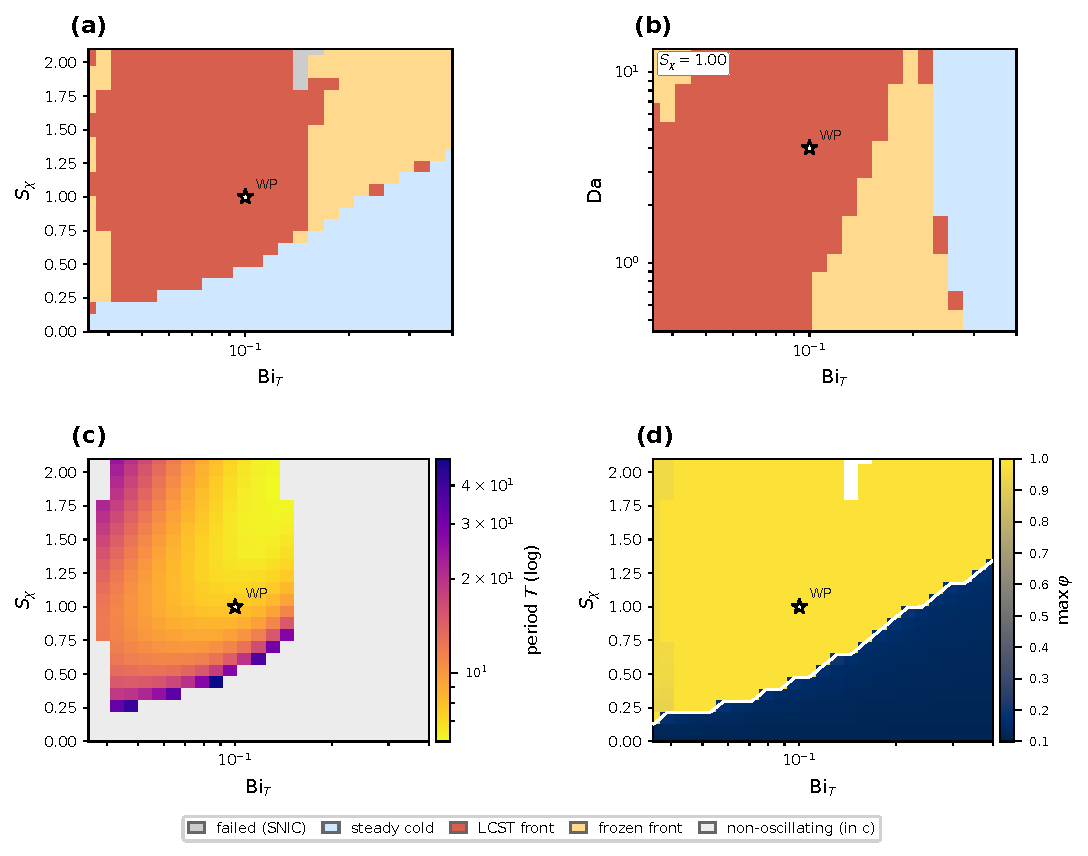
\includegraphics[width=\textwidth]{fig2.pdf}
  \caption{Phase diagram of the realized PDE attractors at the
    default working-point reactivity, from a $25\times25$ default-IC
    sweep.  Star: working point (WP); the bottom legend lists every
    regime present anywhere in panels (a)/(b).
    \textbf{(a)}~Regime classification on $(\Bi_T,S_\chi)$.  Light-grey
    cells (\textit{failed}) mark integrator divergences along the
    saddle--node-on-invariant-circle (SNIC) boundary at large
    $S_\chi$, where the cycle period diverges past the integration
    window.
    \textbf{(b)}~Regime classification on $(\Bi_T,\Da)$ at
    $S_\chi=1.00$, confirming that the LCST-front regime persists
    over a decade in reactivity.
    \textbf{(c)}~Surface oscillation period $T_\mathrm{PDE}$ in the
    LCST-front regime, drawn on a logarithmic colour scale to expose
    the SNIC divergence at the upper- and lower-$S_\chi$ boundaries.
    Light-grey background cells are non-oscillating (steady cold or
    frozen front); see (a) for their classification.
    \textbf{(d)}~Peak polymer fraction $\max_{(\xi,t)}\varphi$.  The
    white contour marks the LCST threshold $\varphi=0.5$ and tracks
    the (a) cold-vs-front boundary, providing an independent check
    on the regime classifier.
  }
  \label{fig:fig4_phase}
\end{figure*}

Figure~\ref{fig:fig_all_regimes} shows the spatiotemporal fields
$J(\xi,t)$, $\theta(\xi,t)$ and the surface and centre $J(t)$ traces
for one representative point per attractor.

The cold-swollen state [Fig.~\ref{fig:fig_all_regimes}(a--c)] is
spatially uniform but is not at the bath temperature: the Arrhenius
source and the surface heat loss equilibrate at a homogeneous
profile [$\theta\!\simeq\!6.9$, $J\!\simeq\!1.18$,
$\varphi\!\simeq\!0.13$ at the representative point]. The LCST
coupling $S_\chi\theta\varphi^2$ is too weak at this $S_\chi$ to
push $\chi_\mathrm{eff}$ past the spinodal, so $\varphi$ remains
well below the LCST threshold and no front is nucleated.

The LCST-front cycle [Fig.~\ref{fig:fig_all_regimes}(d--f)] has a
two-zone structure.  The outer shell ($\xi\!\in\![0.885,\,1]$ at the
working point) cycles between the swollen state ($J\!\sim\!1.4$) and
the collapsed state ($J\!\sim\!0.15$) with period
$T\!\simeq\!8\text{--}11$.  The inner core ($\xi<0.885$) stays at
$J\!\simeq\!1.39$ throughout the cycle.  The temperature field tracks
the asymmetry: $\theta_\mathrm{surf}$ swings between $\sim\!1.5$ and
$\sim\!4.8$ each cycle, while $\theta_\mathrm{centre}$ is held nearly
constant at $\theta_\mathrm{centre}\!\simeq\!3.2$ by heat conduction
from the warm shell.

The frozen-front state [Fig.~\ref{fig:fig_all_regimes}(g--i)] is
stationary in time but strongly heterogeneous in space, with three
regions: a super-swollen interior ($J\!\simeq\!4$,
$\varphi\!\simeq\!0.04$) for $\xi\!\lesssim\!0.91$, a narrow
collapsed band at $\xi\!\simeq\!0.92$ where $J$ drops to
$\simeq\!0.15$ and $\varphi$ rises to $\simeq\!0.98$, and a
super-swollen surface layer ($J\!\simeq\!2.9$--$3.2$) for
$\xi\!\gtrsim\!0.93$.
Two mechanisms combine to produce this profile. First, at
$\Bi_T\!=\!0.18$ the surface heat flux is large enough to clamp the
band's surface side below the re-ignition threshold, locking the
cycle of Sec.~\ref{sec:lcst_front_mechanism} in phase~3. Second, at
$S_\chi\!=\!1.5$ the LCST coupling $S_\chi\theta\varphi^2$ pushes
$\chi_\mathrm{eff}$ so high that the only off-collapse solution of
$\mu(J,\theta)\!=\!\mu_b$ is the dilute branch of the
Flory--Huggins free energy, on which the elastic
$\Omega_e(J\!-\!1/J)$ contribution balances the reduced
$\chi_\mathrm{eff}\varphi^2$ at small $\varphi$. The textbook
``two-zone'' frozen front with a cold-swollen interior and a
collapsed shell is therefore not realised in this model: the bulk
either oscillates (LCST-front cycle) or migrates onto the same
dilute branch that will reappear as the hot-runaway attractor in
Sec.~\ref{sec:multistability}.  A fourth attractor, the hot-runaway hidden state, is
reached only from non-default ICs and is analysed in
Sec.~\ref{sec:multistability} (see Fig.~\ref{fig:fig_manifold}).

\begin{figure*}[tbp]
  \centering
  
\includegraphics[width=\textwidth]{fig3.pdf}
  \caption{Spatiotemporal structure of the three default-IC
    attractors, organised into three rows of three panels each.
    Within every row the columns show, from left to right, the
    $J(\xi,t)$ kymograph, the $\theta(\xi,t)$ kymograph, and the
    time-mean spatial profile $\langle J(\xi)\rangle_t$ with a grey
    min/max envelope band; the grey dotted horizontal line marks the
    LCST threshold $J=\varphi_{p0}/0.5\!\simeq\!0.30$, so any region
    of the profile dropping below it has crossed LCST.
    All three rows show $t\in[0,80]$ so the relaxation from the
    default cold IC onto each attractor is visible in the
    kymographs; the time-mean profile in the right column is
    computed over the post-transient sub-window $t\in[40,80]$ to
    avoid IC bias.
    \textbf{(a--c)}~Cold-swollen steady state at $\Bi_T=0.10$,
    $S_\chi=0.20$; (b) shows $\theta$ rising from the IC value
    $\theta_0\!=\!0$ to the homogeneous reaction--cooling balance
    $\theta\!\simeq\!6.9$ within $t\!\lesssim\!30$, while
    $\varphi$ stays well below the LCST everywhere.
    \textbf{(d--f)}~LCST-front oscillation at the working point
    ($\Bi_T=0.10$, $S_\chi=1.00$); cycles develop from the cold IC
    and reach stable amplitude by $t\!\sim\!30$. The envelope in
    (f) widens from a thin core ($\xi<0.885$, where the trace stays
    above LCST) to the surface shell, where $J$ swings between
    $\sim\!1.4$ and $\sim\!0.15$ each cycle.
    \textbf{(g--i)}~Frozen partial-collapse front at $\Bi_T=0.18$,
    $S_\chi=1.50$; the collapsed band forms within $t\!\sim\!20$
    and locks at $\xi\!\simeq\!0.92$. Panel (i) shows the steady
    three-region profile (super-swollen interior, thin collapsed
    band, super-swollen surface layer); see
    Sec.~\ref{sec:phasediagram} for the mechanism.
    The fourth attractor (hot-runaway hidden state) is accessed
    only from non-default ICs and is shown in
    Fig.~\ref{fig:fig_manifold}.
  }
  \label{fig:fig_all_regimes}
\end{figure*}

\subsection{A relaxation oscillator on a spatially-generated slow
manifold}
\label{sec:lcst_front_mechanism}

The LCST-front cycle is a relaxation oscillator with two
distinguishing features: (i)~the fast variable is mechanical ($J$),
the slow variables are thermal and chemical ($\theta$, $u$); and
(ii)~the slow manifold is generated by the spatial structure of the
gel rather than by an autonomous 0D nonlinearity.  Each cycle
traverses two stable branches of this manifold connected by fast
jumps, and the period is dominated by the slowest of the four phases.

\paragraph{Fast--slow decomposition.}  At the working point the
mechanical relaxation timescale set by the dimensionless mobility
$\Ms_0$ is roughly two orders of magnitude shorter than the thermal
($1/\Bi_T$) and reactant-supply ($1/\Bi_c$) timescales.  Numerically,
the speed
$|d(\theta_\mathrm{surf}, J_\mathrm{surf})/dt|$ along the limit cycle
[Fig.~\ref{fig:fig2_mechanism}(b)]
varies by a factor of $\sim\!600$ between the slow drifts and the
fast jumps.  We may therefore treat $J$ as a fast variable and follow
the standard relaxation-oscillator construction.

\paragraph{Spatially generated slow manifold.}
Quasi-static balance of the surface mechanical equation with the
Robin boundary condition $\Bi_\mu(\mu - \mu_b) = 0$ gives the locus
\begin{equation}
  \mu(J,\theta) \;=\; \mu_b
  \label{eq:slow_manifold}
\end{equation}
in the $(\theta, J)$ plane.  The Flory--Huggins--Rehner free energy
is non-monotonic in $J$ for sufficiently large $\chi_\mathrm{eff}=
\chi_\infty + S_\chi\theta + \chi_1\varphi$ (above the LCST), so this
locus has the canonical S-shape
[Fig.~\ref{fig:fig2_mechanism}(a)]: an upper \emph{swollen} branch
($J \gtrsim 0.8$) for $\theta \le \theta_\mathrm{up}$, a lower
\emph{collapsed} branch ($J \lesssim 0.2$) for
$\theta \ge \theta_\mathrm{lo}$, and a saddle (unstable middle
branch) connecting the two folds.  At the working point,
$\theta_\mathrm{lo}\!\simeq\!0.85$ and
$\theta_\mathrm{up}\!\simeq\!3.18$, defining a bistable region
$\theta\in[\theta_\mathrm{lo},\theta_\mathrm{up}]$ in surface
temperature.  Crucially, this slow manifold lives at the surface and
is enforced by the surface BC; the bulk is buffered away from it by
transport. The contrast is made visible in
Fig.~\ref{fig:fig2_mechanism}(b): the surface trajectory traverses
the entire S-curve between the two folds, while the centre trajectory
(inset) is a small loop confined to the swollen branch's interior at
$(\theta\!\approx\!3.24, J\!\approx\!1.50)$, two orders of magnitude
smaller in extent and never touching the manifold. A 0D
homogeneous-state reduction has no analog of this manifold, since
$\mu = \mu_b$ would have to be imposed everywhere simultaneously
together with the heat and reactant balances
(Sec.~\ref{sec:lsa_vs_nl}).

\paragraph{Cycle traversal.}  The PDE limit cycle, projected onto
$(\theta_\mathrm{surf}, J_\mathrm{surf})$, traces the slow manifold's
two stable branches connected by near-vertical fast jumps
[Fig.~\ref{fig:fig2_mechanism}(b)].
We label four canonical phases:
\begin{enumerate}
\item \textbf{Ignition (slow, on swollen branch).}  The surface
  starts at the cold end of the swollen branch
  ($\theta\!\simeq\!1.5$, $J\!\simeq\!1.4$) with abundant reactant
  ($u_\mathrm{surf}\!\simeq\!1$).  A small thermal fluctuation
  amplifies the Arrhenius factor; the heat source $\Da\,J\Rhat$
  exceeds the surface heat loss $\Bi_T\theta_\mathrm{surf}$ and
  $\theta_\mathrm{surf}$ rises monotonically.
\item \textbf{Collapse (fast).}  As $\theta_\mathrm{surf}$ exceeds
  the upper-fold value, the swollen branch ceases to exist; $J$
  falls rapidly along the fast manifold from $J\!\sim\!0.8$ to
  $J\!\sim\!0.15$ over a small fraction of the cycle period.
\item \textbf{Quenching (slow, on collapsed branch).}  With
  $\varphi\!\sim\!1$ in the collapsed shell the diffusion factor
  $D(\varphi)\propto(1-\varphi)^2$ drops by three orders of magnitude
  and the catalyst-accessibility factor $(1-\varphi)^{m_\mathrm{act}}$
  by ten or more, throttling reactant supply and quenching the
  chemistry. The Robin BC pins
  $u(\xi\!=\!1)$ near the bath value, but inside the closed shell
  the reactant field is several decades lower
  [Fig.~\ref{fig:fig2_mechanism}(c)] and the heat source effectively
  vanishes; $\theta_\mathrm{surf}$ then relaxes towards the bath
  temperature on the surface heat-loss timescale $1/\Bi_T$. Phase 3
  is generally the longest phase of the cycle.
\item \textbf{Re-swelling (fast).}  When $\theta_\mathrm{surf}$
  falls below the lower-fold value, the collapsed branch terminates
  and $J$ jumps back up to the swollen branch.  The diffusion
  barrier reopens, the bath rapidly resupplies reactant, and the
  cycle returns to phase~1.
\end{enumerate}
The slow drifts (phases 1 and 3) and the fast jumps (phases 2 and 4)
are resolved on the limit cycle as differently-coloured segments
[Fig.~\ref{fig:fig2_mechanism}(b)] and on the reactant kymograph
[Fig.~\ref{fig:fig2_mechanism}(c)] as alternating bands of high and
low $u$ at the surface. The corresponding $J(\xi,t)$ and
$\theta(\xi,t)$ fields at the working point are shown explicitly in
Fig.~\ref{fig:fig_all_regimes}(d,e).

\paragraph{Self-limiting collapse.}  The same $\varphi$-dependent
diffusion barrier that quenches the reaction at the surface during
phase~3 also prevents collapse from invading the gel interior.  The
LCST front penetrates only to
$\xi_\mathrm{LCST}\!\simeq\!0.885$ at the working point; the inner
$88.5\%$ of the slab never crosses the LCST and remains swollen
throughout the cycle.  This barrier explains why the classifier-
allowed regimes \emph{globally collapsed steady} and \emph{globally
collapsing oscillation} are absent from the $1000$ default-IC
simulations of Sec.~\ref{sec:phasediagram}: once any portion of the
gel collapses, the inner region is shielded from further reactant
supply and cannot ignite.  The same mechanism is, in this sense, a
self-limiting protective feature of this class of thermo-LCST gel
against runaway global collapse despite the strongly exothermic
Arrhenius
kinetics~\cite{FrankKamenetskii1969,Uppal1974}.

\paragraph{Period structure.} Across the LCST-front regime
[Fig.~\ref{fig:fig4_phase}(c), Fig.~\ref{fig:fig2_mechanism}(c)],
the cycle period $T_\mathrm{PDE}$ takes its minimum value
$\simeq\!6$ in the upper portion of the LCST-front region just
inside the SNIC exit, and diverges at both the upper- and lower-
$S_\chi$ boundaries, where the cycle is destroyed through a
saddle--node-on-invariant-circle (SNIC) bifurcation analyzed in
Sec.~\ref{sec:lsa_vs_nl}. The cooling timescale $1/\Bi_T$ sets the
order of magnitude of the period, but $T_\mathrm{PDE}$ is not a
single power law of $\Bi_T$: phase~3 is also controlled by the
residual interior heat conduction and by the timescale at which the
surface BC restores $u_\mathrm{surf}$ after the diffusion barrier
reopens.

\begin{figure*}[tbp]
  \centering
  
\includegraphics[width=\textwidth]{fig4.pdf}
  \caption{Anatomy of the LCST-front relaxation cycle at the
    working point.
    \textbf{(a)}~Slow-manifold geometry. Heatmap of
    $\mu(J,\theta)-\mu_b$ in the $(\theta,J)$ plane (saturated at
    $\pm 0.6$ to expose the relevant region) with the black
    contour $\mu(J,\theta)=\mu_b$ overlaid; this contour is the
    slow manifold, a level set of the Flory--Huggins--Rehner
    chemical potential at the bath value, and is enforced at
    $\xi\!=\!1$ by the Robin BC. Open circles mark the upper and
    lower folds.
    \textbf{(b)}~PDE limit cycles in the same coordinates. The
    surface trajectory ($\xi\!=\!1$, speed-coloured on a log
    scale) traverses the full S-curve between the folds, with
    $\sim\!600\times$ variation between the slow drifts on the
    swollen/collapsed branches and the near-vertical fast jumps;
    the four phases (ignition, collapse, quenching, re-swelling)
    are read off directly from the cycle topology and segment
    colour. The grey faint S-curve is reproduced from (a) as a
    reference. The inset shows the centre trajectory
    ($\xi\!=\!0$): a small loop confined to the swollen branch's
    interior, two orders of magnitude smaller than the surface
    cycle. The contrast is the §IV.B
    ``spatially generated slow manifold'' argument made visible:
    the manifold is a surface phenomenon, the bulk is buffered
    away from it.
    \textbf{(c)}~Reactant kymograph $u(\xi,\tau)$ on a log scale
    over five cycles. The thin bright band at $\xi\!\to\!1$ is
    the surface boundary layer pinned by the Robin BC near the
    bath value; inside the collapsed shell the field is several
    decades lower because reactant cannot replenish past the
    closed diffusion barrier. The white dashed line at
    $\xi_\mathrm{LCST}\!\simeq\!0.885$ is the innermost $\xi$
    that ever crosses the LCST; below it lies the polymer-
    shielded core that the front never invades.
    \textbf{(d)}~Period scaling $T_\mathrm{PDE}$ vs $1/\Bi_T$
    across all oscillating cells; colour encodes $S_\chi$. Dashed
    line: log-log fit on the central band
    $S_\chi\!\in\![0.30,1.05]$; dotted: the reference
    $T=1/\Bi_T$. The cooling timescale sets the order of
    magnitude but is not a single power-law collapse variable
    because phase 3 also depends on the diffusion-barrier release
    time.
  }
  \label{fig:fig2_mechanism}
\end{figure*}

\FloatBarrier

\subsection{Linear stability is necessary but not sufficient}
\label{sec:lsa_vs_nl}

Section~\ref{sec:lcst_front_mechanism} showed that the LCST-front
attractor is a relaxation cycle whose slow manifold is generated by
the surface boundary condition together with the $\varphi$-dependent
diffusion barrier.  No spatially uniform reduction can produce that
manifold: at the surface the locus $\mu(J,\theta)=\mu_b$ is enforced
by the Robin BC, while in the interior the same locus is irrelevant
because the bulk equilibrium is buffered by transport.  Linear
stability of an available homogeneous branch is therefore at best a
\emph{necessary} condition for the PDE to oscillate; it cannot be
sufficient because the cycle traverses two branches of a slow
manifold that does not exist in the 0D reduction.  This subsection
makes the necessary-condition statement quantitative on two
complementary axes: (i)~where the homogeneous SS even exists as a
real root, and (ii)~how the cycle is destroyed at the parameter-
plane boundaries of the LCST-front regime.

\paragraph{Existence of the homogeneous swollen branch (analytic).}
The 0D steady-state system \eqref{eq:lsa_ss} admits an explicit
parameterization: at any pair $(J,\theta)$ with $J>\varphi_{p0}$,
the two SS conditions solve in closed form for the dependent control
parameters,
\begin{equation}
  S_\chi(J,\theta) =
    \frac{\mu_b - \mu_{\mathrm{base}}(J,\theta)}{\theta\,\varphi^2},
  \qquad
  \Bi_T(J,\theta) = \frac{K(J,\theta)}{\theta\,(1+K/\Bi_c)},
  \label{eq:ss_param_inv}
\end{equation}
where $\mu_{\mathrm{base}}$ is the part of $\mu$ that excludes the
$S_\chi\theta\,\varphi^2$ coupling and
$K(J,\theta)=\Da\,J\,(1-\varphi)^{m_\mathrm{act}}\,T(\theta)$.  The
entire 0D SS surface is therefore the image of the $(J,\theta)$
plane under \eqref{eq:ss_param_inv}, and the saddle--node fold locus
in $(\Bi_T, S_\chi)$ is exactly the image of the curve
$\det\partial(F_1,F_2)/\partial(J,\theta)=0$.  Numerically that
locus is a single connected component in $(J,\theta)$; under the map
\eqref{eq:ss_param_inv} it self-folds in $(\Bi_T, S_\chi)$ into two
branches meeting at a Whitney cusp at
$(\Bi_T,S_\chi)\!\simeq\!(0.43, 2.17)$ — a cusp catastrophe in the
homogeneous-SS surface.

Counting the real roots of \eqref{eq:lsa_ss} cell-by-cell on a
$360\times240$ grid in $(\Bi_T, S_\chi)$ via the closed-form inverse
\eqref{eq:ss_param_inv} (one sign-change scan per cell along $J$,
exact and ${\sim}10^{2}\times$ faster than fsolve) gives
Fig.~\ref{fig:fig_lsa_vs_nl}(a).  The displayed plane decomposes into
$\sim\!37\%$ \emph{swollen-only}, $\sim\!51\%$ \emph{collapsed-only},
and $\sim\!11\%$ \emph{bistable} (3 roots: 2 stable plus 1 saddle);
exactly $0\%$ of cells have $2$ roots.  This odd-only multiplicity
is forced by the fold topology — any horizontal line in
$(\Bi_T, S_\chi)$ at fixed $S_\chi$ crosses the two fold arcs an
even number of times, giving root counts $1,3,5,\ldots$.  The
default working point $(\Bi_T=0.10,S_\chi=1.0)$ and the canonical
C-cell $(\Bi_T=0.059,S_\chi=1.80)$, both used elsewhere in this
section, sit deep inside the ``collapsed-only'' region: at neither
point does the swollen homogeneous SS that one would linearise about
exist as a real root, so a 0D LSA about the swollen branch is
structurally unavailable.  The PDE nevertheless finds the LCST-front
cycle there.  The mismatch is the necessary-but-not-sufficient
statement made geometric: the spatially-generated slow manifold of
Sec.~\ref{sec:lcst_front_mechanism} continues to exist past the
saddle--node fold of the homogeneous problem because its swollen
branch is enforced \emph{at the surface} by the Robin BC, not
required to coexist with bulk reactant balance.


\paragraph{SNIC scaling at the upper-$S_\chi$ exit.}
At the upper-$S_\chi$ boundary of the LCST-front regime
[Fig.~\ref{fig:fig4_phase}(c),
Fig.~\ref{fig:fig2_mechanism}(d)], the cycle period diverges as
$S_\chi\to S_\chi^{(c)}$ from below.  We test the period scaling
along a 1D slice through this boundary against the two canonical
infinite-period scenarios
\begin{equation}
  T_\mathrm{SNIC}(S_\chi)\propto (S_\chi^{(c)}-S_\chi)^{-1/2},
  \qquad
  T_\mathrm{hom}(S_\chi)\propto -\ln(S_\chi^{(c)}-S_\chi),
  \label{eq:snic_vs_hom}
\end{equation}
using the same 1D scan [Fig.~\ref{fig:fig_lsa_vs_nl}(b)].  A two-
parameter least-squares fit of $T_\mathrm{PDE}(S_\chi)$ on the
bracket $S_\chi\in[1.10, 1.32]$ yields a SNIC residual sum of
squares $\mathrm{RSS}_\mathrm{SNIC}=0.068$ versus
$\mathrm{RSS}_\mathrm{hom}=0.152$, with the SNIC fit giving the
critical value $S_\chi^{(c)}\!\approx\!1.34$.  The SNIC inverse-
square-root law captures the data more than twice as well as the
homoclinic log law, consistent with the cycle being destroyed by
the collision of a saddle and a node on the limit cycle rather than
by a homoclinic orbit hitting a saddle off the cycle.  In either
reading the cycle's disappearance is a global topological event in
the surface $(\theta_\mathrm{surf}, J_\mathrm{surf})$ slow-manifold
plane and not a local linear bifurcation of any single homogeneous
branch — the expected signature of a relaxation oscillator on a
spatially generated slow manifold.

\begin{figure*}[tbp]
  \centering
  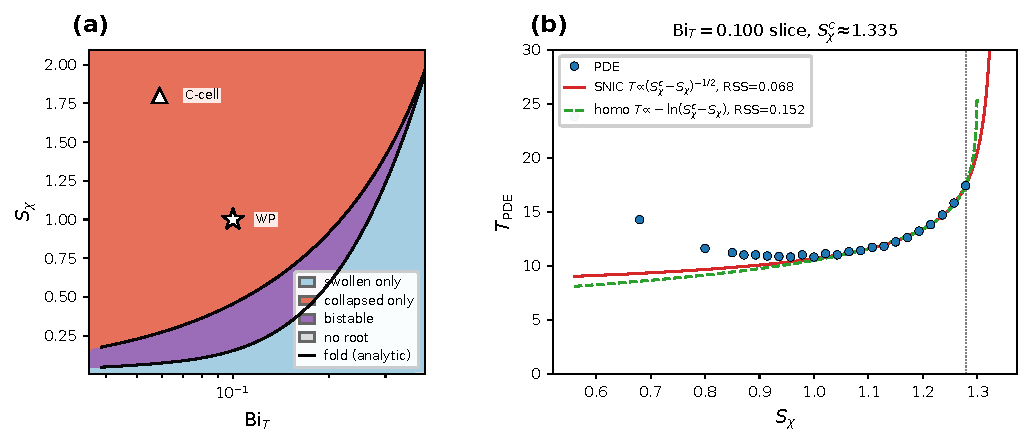
\includegraphics[width=\textwidth]{fig5.pdf}
  \caption{Necessary-but-not-sufficient evidence on
    $(\Bi_T, S_\chi)$.
    \textbf{(a)}~Real-root multiplicity of the homogeneous-SS
    system \eqref{eq:lsa_ss}, computed by the closed-form parameter
    inversion \eqref{eq:ss_param_inv} (1D sign-change scan along
    $J$, $360\times 240$ pixels).  Colours: swollen only (sky blue),
    collapsed only (terra cotta), bistable / 3 roots (purple), no
    root in the displayed window (light grey).  The black analytic
    curve is the saddle--node fold locus, the image of
    $\det\partial(F_1,F_2)/\partial(J,\theta)=0$ under
    \eqref{eq:ss_param_inv}; it self-folds into two arcs meeting at
    a Whitney cusp at $(\Bi_T,S_\chi)\!\simeq\!(0.43,2.17)$.  White
    star: working point; white triangle: C-cell.
    \textbf{(b)}~Period-divergence scaling at the upper-$S_\chi$
    exit.  Open circles: PDE cycle period along a 1D scan in
    $S_\chi$ at fixed $\Bi_T$.  Solid line: SNIC fit
    $T\propto(S_\chi^{(c)}\!-\!S_\chi)^{-1/2}$
    ($S_\chi^{(c)}\!\approx\!1.34$, $\mathrm{RSS}=0.068$).  Dashed
    line: homoclinic fit
    $T\propto-\ln(S_\chi^{(c)}\!-\!S_\chi)$ ($\mathrm{RSS}=0.152$,
    same window).  The SNIC law captures the divergence
    ${\sim}2\times$ better than the homoclinic law.
  }
  \label{fig:fig_lsa_vs_nl}
\end{figure*}

\FloatBarrier

\paragraph{Summary.}
The 0D linear stability analysis carries a precise but limited
informational content: it identifies the local stability of available
homogeneous branches, but the swollen homogeneous branch fails to
exist over $\sim\!51\%$ of the parameter plane covered here, and even
where it does the cycle that the PDE realises is generically not the
small-amplitude continuation of any homogeneous Hopf bifurcation.
The dominant nonlinear behaviour of this thermo-LCST gel is a
relaxation oscillator on a spatially generated slow manifold, born
and destroyed by global topological events
(Sec.~\ref{sec:lcst_front_mechanism} and
Eq.~\eqref{eq:snic_vs_hom}).  Whether the same parameter plane
harbours a hidden second attractor not visible to either linear
analysis or default-IC numerical scans is settled in
Sec.~\ref{sec:multistability}.

\subsection{A hidden hot-runaway state and the IC-induced
hysteresis prediction}
\label{sec:multistability}

Section~\ref{sec:lsa_vs_nl} closed by asking whether the
collapsed-only region of the parameter plane—where the swollen
homogeneous SS does not exist yet the PDE oscillates—corresponds to
genuine attractor multiplicity of the spatially extended problem.
We resolve this by initial-condition (IC) sweeps at a representative
point in this region, the canonical C-cell at $\Bi_T=0.059$,
$S_\chi=1.80$.

\paragraph{Two co-existing attractors.}
At identical bath conditions and reaction parameters, simulations
initialised in different regions of $(J_0, \theta_0)$ space converge
to one of two qualitatively distinct attractors
[Fig.~\ref{fig:fig_manifold}(c)]: (i)~the LCST-front cycle of
Sec.~\ref{sec:lcst_front_mechanism}, with bulk-mean
$\langle J\rangle\!\approx\!2$,
$\langle\theta\rangle\!\approx\!2$, and (ii)~a previously-unreported
\emph{hot-runaway} steady state with
$\langle J\rangle\!\approx\!5$,
$\langle\theta\rangle\!\approx\!12$.  The two attractors differ by
$\Delta\langle J\rangle\!\approx\!3.3$ and
$\Delta\langle\theta\rangle\!\approx\!10$, far beyond any numerical
tolerance, so the bistability is genuine.

\paragraph{Spatial structure and mechanism of the hot-runaway state.}
The hot-runaway state [Fig.~\ref{fig:fig_manifold}(b)] is spatially
uniform with $J\!\simeq\!5.2$, $\theta\!\simeq\!12$,
$\varphi\!\simeq\!0.026$, and a thin reaction layer at the surface
where reactant is consumed almost entirely
($u_\mathrm{surf}\!\sim\!10^{-7}$).  The mechanism is diffusion-
limited combustion: the high-$\theta$ Arrhenius factor exceeds
$10^5$ and burns through any reactant in the boundary layer, but
the surface BC continues to deliver reactant at the diffusion-
limited rate $\Bi_c$.  The gel remains super-swollen because the
high-$J$ Flory--Huggins minimum coexists with the collapsed minimum
whenever $\chi_\mathrm{eff}$ is sufficiently large; at
$\varphi\!\sim\!0.026$ the $\chi_\mathrm{eff}\,\varphi^2$ penalty is
negligible and the elastic term $\Omega_e\,(J-1/J)$ becomes the
dominant contribution to the chemical potential.  The choice
between the two Flory--Huggins minima is set by the IC: trajectories
landing in the basin of the swollen branch reach hot-runaway, while
trajectories landing in the basin of the collapsed branch are
ejected to the LCST-front cycle by the surface BC and the
diffusion-barrier feedback.

\paragraph{Basin asymmetry and why the default sweep misses the
runaway.}
A refined IC sweep on a $11\times 11$ grid at the C-cell
[Fig.~\ref{fig:fig_manifold}(c)] places the basin boundary at roughly
$J_0\!\approx\!1.0$, $\theta_0\!\approx\!1$: only ICs in the
upper-left quadrant of $(J_0, \theta_0)$ space (cold, swollen) reach
the cycle.  ICs with any of (i)~$J_0\!\lesssim\!0.4$ (pre-
collapsed), (ii)~$\theta_0\!\gtrsim\!3$ (ignited), or (iii)~
combinations spanning the basin boundary fall into the runaway.
The basin of the cycle covers $\sim\!13\%$ of the IC grid (16 of
the 119 successfully integrated cells of an $11\times 11$ grid
spanning $J_0\in[0.20, 1.30]$, $\theta_0\in[0,10]$), a small
fraction of the total.  This asymmetry explains why the default
cold-IC sweep of Fig.~\ref{fig:fig4_phase} sees only the cycle and
never the runaway: the default cold IC sits well inside the cycle's
basin at every grid point of the parameter sweep.

\paragraph{IC-induced hysteresis: a falsifiable prediction.}
A 1D slice through the basin space gives a quantitative,
experimentally accessible signature of the bistability
[Fig.~\ref{fig:fig_manifold}(d)].  Holding all reaction and bath
parameters fixed at the C-cell value with the initial reactant
loading $u_0=0.5$, we vary the initial thermal pulse $\theta_0$
from $0$ to $6$ for two seed conditions:
\begin{itemize}
\item ``cold'' seed ($J_0=1.30$): initially near the cold-swollen
  homogeneous state.  For $\theta_0$ below the threshold
  $\theta_0^{\!*}\!\approx\!2.4$ the trajectory remains in the
  cycle's basin and
  $\langle J\rangle_\mathrm{late}\!\approx\!2.0$; for $\theta_0$
  above the threshold the seed crosses the basin boundary and
  $\langle J\rangle_\mathrm{late}\!\approx\!5.9$, indistinguishable
  from the runaway state.  The transition is sharp—the discontinuity
  in $\langle J\rangle_\mathrm{late}$ falls within a single
  $\Delta\theta_0=0.25$ sampling step.
\item ``pre-collapsed'' seed ($J_0=0.20$): initialised inside the
  runaway basin; for every $\theta_0$ in the scanned range the
  trajectory terminates in the runaway-type state with
  $\langle J\rangle_\mathrm{late}\!\approx\!4.2\text{--}5.5$,
  independent of $\theta_0$.
\end{itemize}
The split between the two terminal-state curves over the bistable
$\theta_0$ interval $[0, 2.4]$ is the hysteresis signature.
Experimentally, this would manifest as a sharp jump in long-time
gel volume (or temperature) when the initial perturbation magnitude
is varied across $\theta_0^{\!*}$, with no return jump on the
reverse sweep so long as the C-cell parameters are held fixed.
This is a quantitative prediction of the model that the linear
theory does not provide and that distinguishes spatially-extended
thermo-LCST gels from the well-mixed CSTR
analog~\cite{Uppal1974}.

\begin{figure*}[tbp]
  \centering
  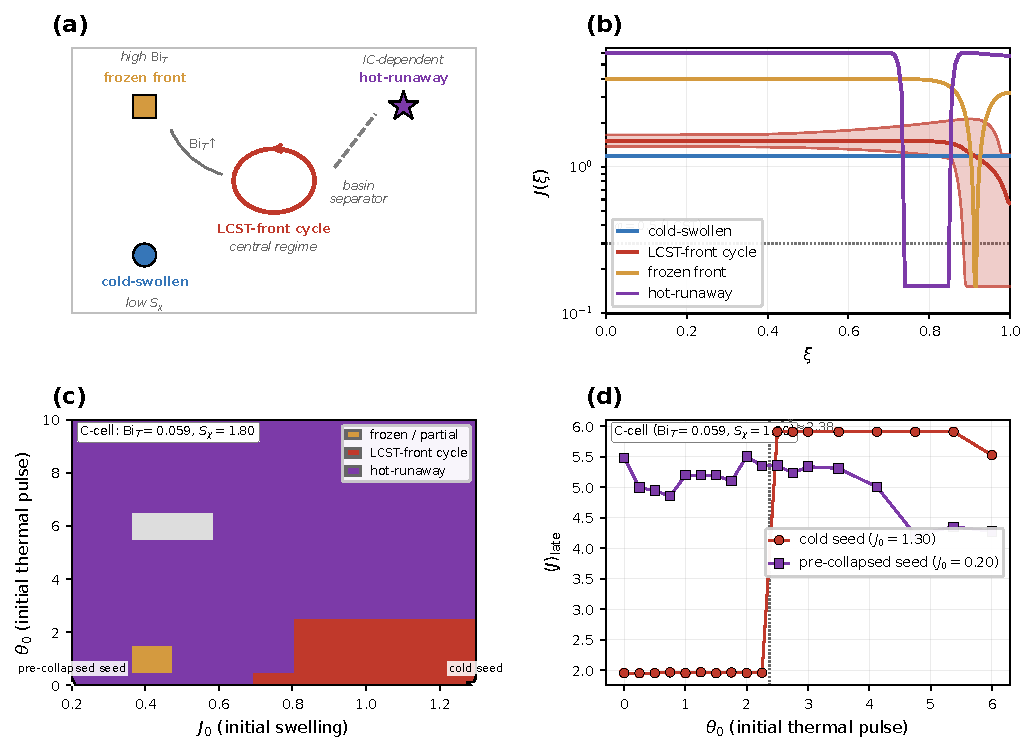
\includegraphics[width=\textwidth]{fig6.pdf}
  \caption{Manifold portrait of the four PDE attractors and IC-
    space evidence at the C-cell.
    \textbf{(a)}~Schematic state-space topology: the LCST-front
    cycle (centre) connects under increasing $\Bi_T$ to the frozen
    front; the cold-swollen and hot-runaway fixed points sit in
    parameter regions disjoint from the cycle, with the
    hot-runaway accessible only across the basin separator at the
    C-cell.
    \textbf{(b)}~Late-time spatial profile $J(\xi)$ for one
    representative trajectory per attractor at its parameter point.
    The LCST-front cycle is shown as the envelope between
    $J_{\min}(\xi)$ and $J_{\max}(\xi)$ (red shading) plus the
    time-mean profile (red curve).  The dotted line marks the LCST
    threshold $\varphi=0.5$, i.e.\ $J=\varphi_{p0}/0.5=0.30$.
    \textbf{(c)}~Refined basin of attraction at the C-cell
    ($\Bi_T=0.059$, $S_\chi=1.80$).  Each pixel of the
    $11\times11$ grid in $(J_0, \theta_0)$ space (fixed $u_0=0.5$)
    is coloured by the long-time attractor reached: red = LCST-
    front cycle, purple = hot-runaway steady state, gold = frozen
    partial collapse, grey = solver failure.  The basin of the
    cycle covers $\sim\!13\%$ of the IC grid; the runaway
    dominates, so the default cold-IC sweep of
    Fig.~\ref{fig:fig4_phase} captures only the cycle.
    \textbf{(d)}~IC-induced hysteresis.  Long-time bulk-mean
    $\langle J\rangle_\mathrm{late}$ vs the initial thermal pulse
    $\theta_0$ for two seed values of $J_0$.  Cold seed
    ($J_0=1.30$, red) jumps sharply from the cycle to the runaway
    at the basin threshold $\theta_0^{\!*}\!\approx\!2.4$, within a
    single $\Delta\theta_0=0.25$ step; pre-collapsed seed
    ($J_0=0.20$, purple) terminates in the runaway state for every
    $\theta_0$.  The split between the two terminal-state curves
    over the bistable interval is the experimentally accessible
    hysteresis signature.
  }
  \label{fig:fig_manifold}
\end{figure*}

\FloatBarrier

The PDE attractor diagram is therefore richer than the single-IC
sweep of Fig.~\ref{fig:fig4_phase} suggests, and richer than 0D
LSA can predict.  The hot-runaway state is invisible to both linear
analysis and to default-IC numerical scans, and its appearance is
contingent on the structure of the basin of attraction in
initial-condition space.  Combined with the slow-manifold
relaxation cycle of Sec.~\ref{sec:lcst_front_mechanism}, this
completes a four-attractor inventory of the spatially extended
problem (cold-swollen, LCST-front cycle, frozen front,
hot-runaway), whose existence and stability are governed not by
any single homogeneous-state linearisation but by the spatial
coupling between the Flory--Huggins free energy and the
$\varphi$-dependent diffusion barrier.

%% ================================================================
%%  V. CONCLUSION
%% ================================================================
\section{Conclusion}
\label{sec:conclusion}

[Section to be written after the revised Results and Discussion is
finalized.]

\begin{acknowledgments}
[Acknowledgments placeholder.]
\end{acknowledgments}

\begin{thebibliography}{99}
\bibitem{Yoshida2014} R.~Yoshida and T.~Ueki, NPG Asia Mater.\ \textbf{6}, e107 (2014).
\bibitem{Yoshida1996} R.~Yoshida, T.~Takahashi, T.~Yamaguchi, and H.~Ichijo, J.~Am.\ Chem.\ Soc.\ \textbf{118}, 5134 (1996).
\bibitem{Yoshida2010} R.~Yoshida, Adv.\ Mater.\ \textbf{22}, 3463 (2010).
\bibitem{Yashin2006} V.~V.~Yashin and A.~C.~Balazs, Science \textbf{314}, 798 (2006).
\bibitem{Siegel1988} R.~A.~Siegel and B.~A.~Firestone, Macromolecules \textbf{21}, 3254 (1988).
\bibitem{Siegel1993} R.~A.~Siegel, Adv.\ Polym.\ Sci.\ \textbf{109}, 233 (1993).
\bibitem{Zarzycki2020} R.~Zarzycki, J.\ Controlled Release \textbf{317}, 1 (2020).
\bibitem{Boissonade2003} J.~Boissonade, Phys.\ Rev.\ Lett.\ \textbf{90}, 188302 (2003).
\bibitem{BoissonadeDeKepper2011} J.~Boissonade and P.~De~Kepper, Phys.\ Chem.\ Chem.\ Phys.\ \textbf{13}, 4848 (2011).
\bibitem{Flory1953} P.~J.~Flory, \textit{Principles of Polymer Chemistry} (Cornell University Press, Ithaca, 1953).
\bibitem{Heskins1968} M.~Heskins and J.~E.~Guillet, J.\ Macromol.\ Sci.\ A \textbf{2}, 1441 (1968).
\bibitem{Hong2008} W.~Hong, X.~Zhao, J.~Zhou, and Z.~Suo, J.\ Mech.\ Phys.\ Solids \textbf{56}, 1779 (2008).
\bibitem{Yashin2012} V.~V.~Yashin, O.~Kuksenok, P.~Dayal, and A.~C.~Balazs, Rep.\ Prog.\ Phys.\ \textbf{75}, 066601 (2012).
\bibitem{Halperin2015} A.~Halperin, M.~Kr\"oger, and F.~M.~Winnik, Angew.\ Chem.\ Int.\ Ed.\ \textbf{54}, 15342 (2015).
\bibitem{Wu1998} C.~Wu and S.~Wang, Phys.\ Rev.\ Lett.\ \textbf{80}, 4092 (1998).
\bibitem{FrankKamenetskii1969} D.~A.~Frank-Kamenetskii, \textit{Diffusion and Heat Exchange in Chemical Kinetics}, 2nd ed.\ (Plenum, New York, 1969).
\bibitem{Richter2004} A.~Richter, D.~Kuckling, S.~Howitz, T.~Gehring, and K.-F.~Arndt, J.\ Microelectromech.\ Syst.\ \textbf{12}, 748 (2003).
\bibitem{Uppal1974} A.~Uppal, W.~H.~Ray, and A.~B.~Poore, Chem.\ Eng.\ Sci.\ \textbf{29}, 967 (1974).
\bibitem{Onuki1993} A.~Onuki, J.\ Phys.\ Soc.\ Jpn.\ \textbf{62}, 385 (1993).
\bibitem{Bai2023} R.~Bai and Z.~Suo, Macromolecules \textbf{56}, 1187 (2023).
\end{thebibliography}

\appendix

%% ================================================================
%%  Appendix A: Model Construction
%% ================================================================
\section{Model Construction}
\label{app:model}

We formulate a one-dimensional Lagrangian model for the coupled thermo-chemo-poroelastic dynamics of a thermoresponsive gel slab undergoing an exothermic reaction. The primary variables are the local swelling ratio $J(X,t)$, reactant concentration $c(X,t)$, and temperature $T(X,t)$.

\subsection{Kinematics}

Consider a gel slab of reference (as-prepared) half-thickness $H_0$. We adopt a material (Lagrangian) coordinate $X\in[0,H_0]$, with $X=0$ denoting the symmetry plane and $X=H_0$ the free surface. The current position of a material point is $x(X,t)$, and the local volume ratio is
\begin{equation}
  J(X,t) = \frac{\partial x}{\partial X} > 0.
  \label{eq:J_def}
\end{equation}
In one dimension, $J$ is the local swelling ratio. The polymer volume fraction is a dependent variable determined by mass conservation of the network:
\begin{equation}
  \phi(X,t) = \frac{\pp}{J(X,t)},
  \label{eq:phi_J}
\end{equation}
where $\pp$ is the polymer volume fraction in the reference (as-prepared) state; $\pp=0.15$ corresponds to a gel that is $85\%$ solvent by volume at preparation. The current thickness of the slab is
\begin{equation}
  h(t) = x(H_0,t) = \int_0^{H_0} J(X,t)\,dX.
  \label{eq:thickness}
\end{equation}

\subsection{Governing equations}

\subsubsection{Swelling--permeation equation}

The evolution of $J$ is governed by solvent conservation:
\begin{equation}
  \frac{\partial J}{\partial t} = -\frac{\partial Q_s}{\partial X},
  \label{eq:J_evol}
\end{equation}
where $Q_s$ is the solvent flux relative to the polymer network, driven by chemical-potential gradients:
\begin{equation}
  Q_s = -M_s(J,T)\,\frac{\partial \mu_s}{\partial X}.
  \label{eq:Qs}
\end{equation}
Here $M_s(J,T)$ is the permeation mobility and $\mu_s$ is the solvent chemical potential.

\subsubsection{Reactant transport equation}

The reactant concentration $c(X,t)$ (moles per unit current total volume) evolves according to
\begin{equation}
  \frac{\partial (Jc)}{\partial t}
  + \frac{\partial N_c}{\partial X}
  = -J\,R(c,T,J),
  \label{eq:c_evol}
\end{equation}
with the total reactant flux
\begin{equation}
  N_c = c\,Q_s - D_c(J,T)\,\frac{\partial c}{\partial X}.
  \label{eq:Nc}
\end{equation}
The first term represents advective transport by the solvent flow, and the second term Fickian diffusion within the pore fluid. The effective diffusivity $D_c(J,T)$ depends on the local microstructure via $J$.

\subsubsection{Heat equation}

The temperature field satisfies
\begin{multline}
  C_\mathrm{eff}(J)\,\frac{\partial T}{\partial t}
  = \frac{\partial}{\partial X}\!\left(K_T(J)\,\frac{\partial T}{\partial X}\right)
  - \frac{\partial}{\partial X}\!\left(c_p^\ell\,T\,Q_s\right)
  \\
  + (-\Delta H_r)\,J\,R(c,T,J),
  \label{eq:T_evol}
\end{multline}
where $C_\mathrm{eff}(J)$ is the effective volumetric heat capacity,
$K_T(J)$ the effective thermal conductivity, $c_p^\ell$ the solvent
heat capacity per unit volume, and $-\Delta H_r > 0$ the exothermic
reaction enthalpy.  The three right-hand-side terms represent thermal
conduction, enthalpy advection by the solvent flow, and reaction heat
generation, respectively.

\subsection{Free energy and chemical potential}

The Helmholtz free-energy density per unit reference volume is written as
\begin{equation}
  \Psi(J,T) = \Psi_\mathrm{el}(J) + \Psi_\mathrm{mix}(\phi,T)
  + \frac{\kappa_J}{2}\left(\frac{\partial J}{\partial X}\right)^2,
  \label{eq:Psi}
\end{equation}
where $\phi = \pp/J$, and the three contributions are the elastic
energy of the network, the Flory--Huggins mixing energy, and a
gradient-energy regularization.

For the polymer network we adopt a neo-Hookean elastic energy
appropriate for uniaxial swelling in the slab geometry:
\begin{equation}
  \Psi_\mathrm{el}(J) = \frac{G}{2}
  \bigl(J^{2} - 1 - 2\ln J\bigr),
  \label{eq:Psi_el}
\end{equation}
where $G$ is the shear modulus of the reference-state network.
(For the isotropic sphere, the corresponding expression is
$\Psi_\mathrm{el}=\frac{G}{2}(3J^{2/3}-3-2\ln J)$; see
Sec.~\ref{sec:results}.)

The mixing free-energy density takes the standard Flory--Huggins
form~\cite{Flory1953}:
\begin{equation}
  \Psi_\mathrm{mix}(\phi,T)
  = \frac{R_g T}{v_s}
  \Big[(1-\phi)\ln(1-\phi) + \chi(T,\phi)\,\phi(1-\phi)\Big],
  \label{eq:Psi_mix}
\end{equation}
with $R_g$ the gas constant, $v_s$ the solvent molar volume, and
the Flory--Huggins interaction parameter
\begin{equation}
  \chi(T,\phi) = \chi_0(T) + \chi_1\,\phi.
  \label{eq:chi}
\end{equation}
The temperature-dependent part $\chi_0(T)$ encodes the LCST
behavior of the gel; $\chi_1$ captures the leading
concentration dependence.

The solvent chemical potential is obtained as
$\mu_s = v_s\,\partial\Psi/\partial(1-\phi)\cdot
\partial(1-\phi)/\partial J$~\cite{Hong2008}.  Evaluating this
derivative yields the mixing contribution
\begin{equation}
  \frac{\mu_\mathrm{mix}}{R_g T/v_s}
  = \ln(1-\phi) + \phi + \chi(T,\phi)\,\phi^2,
  \label{eq:mu_mix}
\end{equation}
and the elastic contribution
\begin{equation}
  \frac{\mu_\mathrm{el}}{R_g T/v_s}
  = \frac{G\,v_s}{R_g T}
  \bigl(J - J^{-1}\bigr).
  \label{eq:mu_el}
\end{equation}
The full chemical potential, including the gradient-energy
regularization, is
\begin{equation}
  \mu_s = \mu_\mathrm{mix}(J,T) + \mu_\mathrm{el}(J)
  - \kappa_J\,\frac{\partial^2 J}{\partial X^2}.
  \label{eq:mu_s}
\end{equation}

\subsection{Reaction kinetics}

The volumetric reaction rate takes the Arrhenius form modulated by a collapse-dependent accessibility factor:
\begin{equation}
  R(c,T,J) = k_0\,c^n\,\exp\!\left(-\frac{E_a}{R_g T}\right) a(J),
  \label{eq:R}
\end{equation}
where $k_0$ is the pre-exponential factor, $n$ the reaction order, and $E_a$ the activation energy.

The activity factor $a(J)$ models the suppression of reaction due to reduced free solvent volume upon collapse:
\begin{equation}
  a(J) = \left(1 - \frac{\pp}{J}\right)^{m_\mathrm{act}}
  = (1-\phi)^{m_\mathrm{act}}.
  \label{eq:aJ}
\end{equation}
When the gel collapses ($J\to\pp$, $\phi\to 1$), the activity vanishes, shutting off the reaction.

The effective transport coefficients similarly depend on the microstructure:
\begin{align}
  D_c(J) &= D_0\left(1-\frac{\pp}{J}\right)^{m_\mathrm{diff}}, \label{eq:Dc} \\
  M_s(J) &= M_0\left(1-\frac{\pp}{J}\right)^{m_\mathrm{mob}}, \label{eq:Ms}
\end{align}
so that both solute diffusion and solvent permeation are suppressed in the collapsed state.

\subsection{Boundary conditions}

At the symmetry plane $X=0$:
\begin{equation}
  Q_s = 0, \qquad N_c = 0, \qquad \frac{\partial T}{\partial X} = 0.
  \label{eq:bc_sym}
\end{equation}

At the free surface $X=H_0$:

\paragraph{Solvent exchange.}
A Robin-type condition couples the surface chemical potential to the bath:
\begin{equation}
  Q_s = L_\mu\!\left(\mu_s - \mu_\mathrm{bath}\right),
  \label{eq:bc_mu}
\end{equation}
where $L_\mu$ is a surface transfer coefficient. In the limit of rapid equilibration, $\mu_s = \mu_\mathrm{bath}$.

\paragraph{Reactant supply.}
\begin{equation}
  N_c = k_c\,(c - c_b),
  \label{eq:bc_c}
\end{equation}
where $c_b$ is the constant bath concentration.

\paragraph{Heat exchange.}
\begin{equation}
  -K_T\,\frac{\partial T}{\partial X} = h_T\,(T - T_\infty),
  \label{eq:bc_T}
\end{equation}
where $h_T$ is the surface heat-transfer coefficient and $T_\infty$ the ambient temperature.

\paragraph{Mechanical boundary.}
The free surface is traction-free. In the $J$-formulation this is implicitly satisfied by the chemical-potential balance.

%% ================================================================
%%  Appendix B: Nondimensionalization
%% ================================================================
\section{Nondimensionalization}
\label{app:nondim}

\subsection{Scaling}

We introduce the following dimensionless variables. Length is scaled by the reference thickness:
\begin{equation}
  X = H_0\,\tilde{x}, \qquad \tilde{x}\in[0,1].
\end{equation}
The swelling ratio $J$ is already dimensionless. Reactant concentration is normalized by the bath value:
\begin{equation}
  c = c_b\,u.
\end{equation}
Temperature is measured relative to ambient, scaled by the adiabatic reaction temperature rise:
\begin{equation}
  T = T_\infty + \Delta T_*\,\theta,
  \qquad
  \Delta T_* = \frac{(-\Delta H_r)\,c_b}{C_*},
\end{equation}
where $C_*$ is a representative volumetric heat capacity.

The chemical potential is scaled by the thermal mixing energy:
\begin{equation}
  \mu_s = \mu_*\,m, \qquad \mu_* = \frac{R_g T_\infty}{v_s}.
\end{equation}

Time is scaled by the swelling/permeation time:
\begin{equation}
  \tau_s = \frac{H_0^2}{M_0\,\mu_*},
\end{equation}
where $M_0$ is a reference mobility. The solvent and reactant flux scales follow:
\begin{equation}
  Q_s = \frac{H_0}{\tau_s}\,q,
  \qquad
  N_c = \frac{c_b\,H_0}{\tau_s}\,n.
\end{equation}

Material functions are factored as reference value times dimensionless function:
\begin{align}
  M_s &= M_0\,\Ms(J,\theta), &
  D_c &= D_0\,\Ds(J,\theta), \\
  C_\mathrm{eff} &= C_*\,\Cs(J), &
  K_T &= K_*\,\Ks(J).
\end{align}

\subsection{Dimensionless reaction rate}

Defining the reference reaction rate
\begin{equation}
  R_0 = k_0\,c_b^{\,n}\,\exp\!\left(-\frac{E_a}{R_g T_\infty}\right),
\end{equation}
we write $R = R_0\,\Rhat(u,\theta,J)$ with
\begin{equation}
  \Rhat(u,\theta,J)
  = u^n\,a(J)\,
  \exp\!\left[\frac{\Gamma_A\,\theta}{1+\varepsilon_T\,\theta}\right],
  \label{eq:Rhat}
\end{equation}
where
\begin{equation}
  \varepsilon_T = \frac{\Delta T_*}{T_\infty},
  \qquad
  \Gamma_A = \frac{E_a\,\Delta T_*}{R_g\,T_\infty^2}.
  \label{eq:epsT_GammaA}
\end{equation}
When $\varepsilon_T \ll 1$, this simplifies to $\Rhat \approx u^n\,a(J)\,e^{\Gamma_A\theta}$.

\subsection{Dimensionless chemical potential}

The dimensionless chemical potential is
\begin{equation}
  m = m_\mathrm{mix}(J,\theta) + m_\mathrm{el}(J) - \ell^2\,\frac{\partial^2 J}{\partial \tilde{x}^2},
  \label{eq:m_nondim}
\end{equation}
with the interface parameter
\begin{equation}
  \ell^2 = \frac{\kappa_J}{\mu_*\,H_0^2}.
\end{equation}

The mixing part retains the Flory--Huggins form (neglecting the
$T/T_\infty\approx 1+\varepsilon_T\theta\approx 1$ prefactor, valid
when $\varepsilon_T\ll 1$):
\begin{equation}
  m_\mathrm{mix} = \ln(1-\phi) + \phi + \chi(\theta,\phi)\,\phi^2,
  \qquad \phi = \frac{\pp}{J},
  \label{eq:m_mix}
\end{equation}
with the dimensionless interaction parameter
\begin{equation}
  \chi(\theta,\phi) = \chi_\infty + S_\chi\,\theta + \chi_1\,\phi,
  \label{eq:chi_nondim}
\end{equation}
where $\chi_\infty = \chi_0(T_\infty)$ and the thermo-swelling sensitivity is
\begin{equation}
  S_\chi = \Delta T_*\left.\frac{d\chi_0}{dT}\right|_{T_\infty}.
  \label{eq:Schi}
\end{equation}

The elastic contribution follows from Eq.~\eqref{eq:mu_el}:
\begin{equation}
  m_\mathrm{el} = \Omega_e\,(J - J^{-1}),
  \qquad
  \Omega_e = \frac{G\,v_s}{R_g\,T_\infty},
\end{equation}
measuring the network stiffness relative to the thermal mixing energy.

\subsection{Dimensionless governing equations}

Dropping tildes for clarity, the dimensionless system reads:

\paragraph{Swelling equation.}
\begin{equation}
  \frac{\partial J}{\partial t}
  = \frac{\partial}{\partial x}\!\left(\Ms(J,\theta)\,\frac{\partial m}{\partial x}\right),
  \label{eq:J_nondim}
\end{equation}

\paragraph{Chemical potential.}
\begin{equation}
  m = m_\mathrm{mix}(J,\theta) + m_\mathrm{el}(J) - \ell^2\,\frac{\partial^2 J}{\partial x^2},
  \label{eq:m_nondim_box}
\end{equation}

\paragraph{Reactant equation.}
\begin{equation}
  \frac{\partial(J u)}{\partial t}
  + \frac{\partial}{\partial x}\!\left(u\,q - \delta\,\Ds(J,\theta)\,\frac{\partial u}{\partial x}\right)
  = -\Da\,J\,\Rhat(u,\theta,J),
  \label{eq:u_nondim}
\end{equation}
where $q = -\Ms(J,\theta)\,\partial_x m$ and
\begin{equation}
  \delta = \frac{D_0}{M_0\,\mu_*}
\end{equation}
is the ratio of solute diffusion speed to solvent permeation speed.

The Damk\"ohler number, measuring reaction rate relative to swelling rate, is
\begin{equation}
  \Da = \tau_s\,k_0\,c_b^{\,n-1}\,\exp\!\left(-\frac{E_a}{R_g T_\infty}\right).
  \label{eq:Da}
\end{equation}

\paragraph{Heat equation.}
\begin{multline}
  \Cs(J)\,\frac{\partial\theta}{\partial t}
  = \alpha\,\frac{\partial}{\partial x}\!\left(\Ks(J)\,\frac{\partial\theta}{\partial x}\right)
  + \Da\,J\,\Rhat(u,\theta,J)
  \\
  - \alpha\,\Pe_T\,\frac{\partial}{\partial x}\!\left[(\Theta_\infty + \theta)\,q\right],
  \label{eq:theta_nondim}
\end{multline}
with
\begin{equation}
  \alpha = \frac{K_*\,\tau_s}{C_*\,H_0^2} = \frac{\tau_s}{\tau_T},
  \quad
  \Pe_T = \frac{c_p^\ell\,M_0\,\mu_*}{K_*},
  \quad
  \Theta_\infty = \frac{T_\infty}{\Delta T_*},
  \label{eq:thermal_params}
\end{equation}
where $\tau_T = C_*H_0^2/K_*$ is the thermal diffusion time.
When $\Pe_T \ll 1$, the convective term may be dropped.

\paragraph{Constraint.}
\begin{equation}
  \phi = \frac{\pp}{J}.
\end{equation}

\subsection{Dimensionless boundary conditions}

At $x=0$ (symmetry):
\begin{equation}
  q = 0, \qquad
  u\,q - \delta\,\Ds\,u_x = 0, \qquad
  \theta_x = 0.
  \label{eq:bc0_nondim}
\end{equation}

At $x=1$ (free surface):
\begin{align}
  q &= \Bi_\mu\,(m - m_b), \label{eq:bc1_mu} \\
  u\,q - \delta\,\Ds\,u_x &= \Bi_c\,(u - 1), \label{eq:bc1_c} \\
  -\alpha\,\Ks(J)\,\theta_x &= \Bi_T\,\theta, \label{eq:bc1_T}
\end{align}
where the surface Biot numbers for permeation and mass transfer are
\begin{equation}
  \Bi_\mu = \frac{L_\mu\,H_0}{M_0},
  \qquad
  \Bi_c = \frac{k_c\,H_0}{M_0\,\mu_*},
  \label{eq:Bi_mu_c}
\end{equation}
and the thermal exchange number is
\begin{equation}
  \Bi_T = \frac{h_T\,\tau_s}{C_*\,H_0}
  = \alpha\,\frac{h_T\,H_0}{K_*},
  \label{eq:Bi_T}
\end{equation}
which measures the surface heat loss rate directly on the swelling
timescale $\tau_s$.  The standard thermal Biot number
$h_T H_0/K_*=\Bi_T/\alpha$ is recovered by factoring out $\alpha$.

\subsection{Controlling parameter groups}

The oscillatory dynamics are governed by the following dimensionless groups:
\begin{itemize}
  \item $\Da$\,---\,Damk\"ohler number: strength of reaction heat source relative to swelling.
  \item $\alpha = \tau_s/\tau_T$\,---\,thermal diffusion relative to swelling.
  \item $S_\chi$\,---\,thermo-swelling sensitivity: how strongly temperature shifts the interaction parameter.
  \item $\Gamma_A$\,---\,Arrhenius feedback strength.
  \item $\delta$\,---\,solute diffusion to permeation ratio.
  \item $\ell$\,---\,interface regularization length.
  \item $\Bi_c$\,---\,surface reactant Biot number.
  \item $\Bi_T$\,---\,thermal exchange number (surface heat loss on the swelling timescale).
\end{itemize}
Together with the working-point parameters $\pp$ and $\chi_\infty$, these form the minimal set controlling the onset of self-oscillation. In physical terms, oscillation requires that the fast positive feedback (reaction $\to$ heating $\to$ collapse) and the slow negative feedback (collapse $\to$ transport suppression $\to$ cooling $\to$ re-swelling) operate on well-separated time scales.

%% ================================================================
%%  Appendix C: Dispersion Relation Derivation
%% ================================================================
\section{Dispersion Relation Derivation}
\label{app:lsa}

We derive the dispersion matrix $\mathbf A(k)$ introduced in
Eq.~\eqref{eq:dispersion_matrix}.  The $k=0$ matrix $\mathbf A_0$
is obtained by volume-averaging the governing equations over the slab
domain and incorporating the Robin boundary fluxes as lumped
source/sink terms.  The $k^2$ and $k^4$ matrices $\mathbf D_2$ and
$\mathbf D_4$ collect the bulk diffusion contributions from a
point-wise normal-mode analysis; cross-coupling through advection
($u_x\,q$ and $\theta_x\,q$) vanishes identically at the uniform
base state because both $q_0=0$ and the field gradients vanish.

Starting from the mixed
formulation~\eqref{eq:mixed_J}--\eqref{eq:mixed_T}, the chemical
potential entering the swelling flux is
\begin{equation}
  m = f(J,\theta) - \ell^2 J_{\xi\xi},
\end{equation}
with $f(J,\theta)=m_\mathrm{mix}(J,\theta)+m_\mathrm{el}(J)$.
We perturb about the uniform base state with normal modes
$(\widehat J,\widehat u,\widehat\theta)^T e^{\sigma t+ik\xi}$
and define the partial derivatives
\begin{subequations}
\begin{align}
  f_J &= \left.\frac{\partial f}{\partial J}\right|_0, &
  f_\theta &= \left.\frac{\partial f}{\partial \theta}\right|_0,
  \\
  R_J &= \left.\frac{\partial \Rhat}{\partial J}\right|_0, &
  R_u &= \left.\frac{\partial \Rhat}{\partial u}\right|_0,
  \\
  R_\theta &= \left.\frac{\partial \Rhat}{\partial \theta}\right|_0,
\end{align}
\end{subequations}
and the base-state transport coefficients
\begin{subequations}
\begin{align}
  \Ms_0 &= \Ms(J_0,\theta_0), &
  \Ds_0 &= \delta\,\Ds(J_0,\theta_0),
  \\
  \Ks_0 &= \alpha\,\Ks(J_0), &
  \Cs_0 &= \Cs(J_0).
\end{align}
\end{subequations}

The $k=0$ matrix $\mathbf A_0$ contains the reaction and
boundary-exchange terms:
\begin{equation}
  \mathbf A_0 =
  \begin{bmatrix}
    a_{11} & 0 & a_{13} \\
    a_{21} & a_{22} & a_{23} \\
    a_{31} & a_{32} & a_{33}
  \end{bmatrix},
  \label{eq:A0}
\end{equation}
with entries
\begin{subequations}
\label{eq:A0_entries}
\begin{align}
  a_{11} &= -\Bi_\mu f_J, \qquad
  a_{13} = -\Bi_\mu f_\theta, \\
  a_{21} &= \frac{u_0\Bi_\mu f_J
             - \Da(\Rhat_0 + J_0R_J)}{J_0}, \\
  a_{22} &= \frac{-\Bi_c - \Da J_0 R_u}{J_0}, \\
  a_{23} &= \frac{u_0\Bi_\mu f_\theta
             - \Da J_0 R_\theta}{J_0}, \\
  a_{31} &= \frac{\Da(\Rhat_0 + J_0R_J)}{\Cs_0}, \quad
  a_{32} = \frac{\Da J_0 R_u}{\Cs_0}, \\
  a_{33} &= \frac{-\Bi_T + \Da J_0R_\theta}{\Cs_0}.
\end{align}
\end{subequations}
Note that $a_{12}=0$ because the swelling equation does not depend
directly on the reactant concentration.

The $k^2$ contribution collects diffusive transport:
\begin{equation}
  \mathbf D_2 =
  \begin{bmatrix}
    -\Ms_0 f_J & 0 & -\Ms_0 f_\theta \\
    0 & -\Ds_0/J_0 & 0 \\
    0 & 0 & -\Ks_0/\Cs_0
  \end{bmatrix}.
  \label{eq:D2}
\end{equation}
The $(1,1)$ entry $-\Ms_0 f_J$ changes sign when $f_J<0$ (spinodal
region), acting as a negative diffusivity for~$J$.

The only $k^4$ contribution arises from the Cahn--Hilliard
regularization:
\begin{equation}
  \mathbf D_4 =
  \begin{bmatrix}
    -\Ms_0\ell^2 & 0 & 0 \\
    0 & 0 & 0 \\
    0 & 0 & 0
  \end{bmatrix}.
  \label{eq:D4}
\end{equation}
Together, $\mathbf A(k) = \mathbf A_0 + k^2\mathbf D_2 +
k^4\mathbf D_4$ yields a $3\times 3$ eigenvalue problem for each
wavenumber~$k$.


%% ================================================================
%%  Appendix D: Numerical Method
%% ================================================================
\section{Numerical Method}
\label{app:numerics}

We describe a cell-centered finite-volume spatial discretization for the
dimensionless system derived in Appendix~\ref{app:nondim}.  Time
integration uses the implicit BDF method provided by
\textsc{scipy.integrate.solve\_ivp}: the spatial operators below
define the right-hand side of the resulting ODE system (method of
lines).  In the notation below, superscript~$n$ denotes the current
time level and~$n\!+\!1$ the new level; starred quantities
($\Ms_i^*$, $\theta_i^*$, $\Cs_i^*$) are evaluated at the most
recent available state, and $\sharp$-quantities ($J_i^\sharp$,
$u_i^\sharp$) at the values from the preceding fractional stage when
operator splitting is used.

\subsection{Mixed formulation}

To avoid discretizing fourth-order derivatives directly, we introduce the auxiliary variables $m$, $q$, $n$, and $h$ and write the system as
\begin{align}
  J_t + q_x &= 0, & q &= -\Ms(J,\theta)\,m_x, \label{eq:mixed_J} \\
  m &= f(J,\theta) - \ell^2\,J_{xx}, \label{eq:mixed_m} \\
  (Ju)_t + n_x &= -\Da\,J\,\Rhat, & n &= u\,q - \delta\,\Ds(J,\theta)\,u_x, \label{eq:mixed_u} \\
  \Cs(J)\,\theta_t + h_x &= \Da\,J\,\Rhat, & h &= -\alpha\,\Ks(J)\,\theta_x, \label{eq:mixed_T}
\end{align}
where $f(J,\theta) = m_\mathrm{mix}(J,\theta) + m_\mathrm{el}(J)$. This mixed form requires only $C^0$ regularity (no second-derivative continuity) and naturally accommodates Robin boundary conditions.

\subsection{Spatial discretization}

We use a uniform mesh of $N$ cells:
\begin{equation}
  \Delta x = \frac{1}{N},
  \qquad
  x_i = \left(i - \tfrac{1}{2}\right)\Delta x,
  \quad i = 1,\dots,N.
  \label{eq:mesh}
\end{equation}
Face positions are $x_{i+1/2} = i\,\Delta x$ for $i=0,\dots,N$. Cell-centered unknowns are $J_i,\,m_i,\,u_i,\,\theta_i$; face fluxes are $q_{i+1/2},\,n_{i+1/2},\,h_{i+1/2}$.

\subsubsection{Swelling equation}

The conservative update reads
\begin{equation}
  \frac{J_i^{n+1} - J_i^{n}}{\Delta t}
  + \frac{q_{i+1/2}^{n+1} - q_{i-1/2}^{n+1}}{\Delta x} = 0,
  \label{eq:disc_J}
\end{equation}
with the face flux
\begin{equation}
  q_{i+1/2}^{n+1}
  = -\Ms_{i+1/2}^{*}\,
  \frac{m_{i+1}^{n+1} - m_i^{n+1}}{\Delta x}.
  \label{eq:disc_q}
\end{equation}
The face mobility $\Ms_{i+1/2}^{*}$ is evaluated using the harmonic mean
\begin{equation}
  \Ms_{i+1/2}^{*}
  = \frac{2\,\Ms_i^{*}\,\Ms_{i+1}^{*}}{\Ms_i^{*} + \Ms_{i+1}^{*}},
  \label{eq:harm_mean}
\end{equation}
which is more robust than arithmetic averaging for degenerate mobilities.

\subsubsection{Chemical potential}

The discrete chemical potential is
\begin{equation}
  m_i^{n+1}
  = f(J_i^{n+1},\theta_i^{*})
  - \ell^2\,\frac{J_{i+1}^{n+1} - 2J_i^{n+1} + J_{i-1}^{n+1}}{\Delta x^2},
  \label{eq:disc_m}
\end{equation}
where the natural boundary condition $\partial_x J = 0$ is imposed via ghost cells:
\begin{equation}
  J_0^{n+1} = J_1^{n+1}, \qquad J_{N+1}^{n+1} = J_N^{n+1}.
  \label{eq:ghost_J}
\end{equation}

\subsubsection{Reactant equation}

To preserve conservation, we update the product $W_i = J_i\,u_i$:
\begin{equation}
  \frac{W_i^{n+1} - W_i^{n}}{\Delta t}
  + \frac{n_{i+1/2}^{n+1} - n_{i-1/2}^{n+1}}{\Delta x}
  = -\Da\,J_i^{\sharp}\,\Rhat(u_i^{\sharp},\theta_i^{\sharp},J_i^{\sharp}),
  \label{eq:disc_W}
\end{equation}
followed by reconstruction $u_i^{n+1} = W_i^{n+1}/J_i^{n+1}$.

The reactant face flux combines upwind advection and central diffusion:
\begin{equation}
  n_{i+1/2}^{n+1}
  = q_{i+1/2}^{n+1}\,u_{i+1/2}^\mathrm{up}
  - \delta\,\Ds_{i+1/2}^{*}\,
  \frac{u_{i+1}^{n+1} - u_i^{n+1}}{\Delta x},
  \label{eq:disc_n}
\end{equation}
where the upwind value is
\begin{equation}
  u_{i+1/2}^\mathrm{up}
  = \begin{cases}
    u_i^{n+1}, & q_{i+1/2}^{n+1} \ge 0, \\[4pt]
    u_{i+1}^{n+1}, & q_{i+1/2}^{n+1} < 0.
  \end{cases}
  \label{eq:upwind}
\end{equation}
Upwinding is essential to suppress spurious oscillations when advection dominates over diffusion.

\subsubsection{Heat equation}

The thermal update is
\begin{equation}
  \Cs_i^{*}\,\frac{\theta_i^{n+1} - \theta_i^{n}}{\Delta t}
  + \frac{h_{i+1/2}^{n+1} - h_{i-1/2}^{n+1}}{\Delta x}
  = \Da\,J_i^{\sharp}\,\Rhat(u_i^{\sharp},\theta_i^{\sharp},J_i^{\sharp}),
  \label{eq:disc_theta}
\end{equation}
with the heat flux (neglecting enthalpy advection)
\begin{equation}
  h_{i+1/2}^{n+1}
  = -\alpha\,\Ks_{i+1/2}^{*}\,
  \frac{\theta_{i+1}^{n+1} - \theta_i^{n+1}}{\Delta x}.
  \label{eq:disc_h}
\end{equation}

\subsection{Boundary conditions}

At the left boundary ($x=0$):
\begin{equation}
  q_{1/2}^{n+1} = 0,
  \qquad
  n_{1/2}^{n+1} = 0,
  \qquad
  h_{1/2}^{n+1} = 0.
  \label{eq:disc_bc0}
\end{equation}

At the right boundary ($x=1$), the Robin conditions become face fluxes:
\begin{align}
  q_{N+1/2}^{n+1} &= \Bi_\mu\,(m_N^{n+1} - m_b), \label{eq:disc_bc1_q} \\
  n_{N+1/2}^{n+1} &= \Bi_c\,(u_N^{n+1} - 1), \label{eq:disc_bc1_n} \\
  h_{N+1/2}^{n+1} &= \Bi_T\,\theta_N^{n+1}. \label{eq:disc_bc1_h}
\end{align}

\subsection{Time integration}

The primary integration strategy is the method of lines (MOL): the
spatial discretization above defines a system of $4N$ coupled ODEs
that is advanced in time by the variable-order implicit BDF solver
(\textsc{scipy.integrate.solve\_ivp} with \texttt{method='BDF'} and
a precomputed Jacobian sparsity pattern).  Adaptive time stepping
and error control are handled by the library.

For parameter regimes where the BDF solver encounters difficulties,
an alternative IMEX operator-splitting strategy is available, in
which each time step proceeds sequentially:

\paragraph{Stage 1: Swelling $(J,m,q)$.}
Given $(J^n, u^n, \theta^n)$, solve the coupled nonlinear system~\eqref{eq:disc_J}--\eqref{eq:disc_m} for $(J^{n+1}, m^{n+1}, q^{n+1})$ using Newton iteration. The mobility and thermodynamic function $f$ are evaluated at the current iterate $(J^{(k)},\theta^{(k)})$.

\paragraph{Stage 2: Reactant $(W,u)$.}
With $J^{n+1}$ and $q^{n+1}$ known, solve the linear (or mildly nonlinear) system~\eqref{eq:disc_W}--\eqref{eq:disc_n} for $W^{n+1}$, then recover $u^{n+1} = W^{n+1}/J^{n+1}$. Diffusion is treated implicitly; the reaction source may be linearized about the current temperature.

\paragraph{Stage 3: Temperature $(\theta)$.}
With $J^{n+1}$ and $u^{n+1}$ known, solve the implicit heat equation~\eqref{eq:disc_theta}--\eqref{eq:disc_h} for $\theta^{n+1}$. If the Arrhenius source term is stiff, a Newton linearization of the source with respect to $\theta$ is applied.

\subsection{Fully coupled Newton formulation}

For problems requiring tight coupling, the unknowns are assembled
into a single vector
\begin{multline}
  \bm{Y} = (J_1,\dots,J_N,\;m_1,\dots,m_N,\\
  W_1,\dots,W_N,\;\theta_1,\dots,\theta_N)^T
\end{multline}
and the residual vector $\bm{R}(\bm{Y})$ collects all discrete equations~\eqref{eq:disc_J}--\eqref{eq:disc_h} with boundary conditions~\eqref{eq:disc_bc0}--\eqref{eq:disc_bc1_h}. The system is solved by Newton's method:
\begin{equation}
  \bm{J}_\mathrm{ac}\,\delta\bm{Y} = -\bm{R}(\bm{Y}^{(k)}),
  \qquad
  \bm{Y}^{(k+1)} = \bm{Y}^{(k)} + \delta\bm{Y},
\end{equation}
where $\bm{J}_\mathrm{ac}$ is the Jacobian matrix. Because all couplings are local in one dimension, the Jacobian is sparse and banded; its sparsity pattern is precomputed and supplied to the BDF integrator for efficient graph-coloring-based finite-difference Jacobian evaluation.

\subsection{Implementation notes}

\begin{enumerate}
  \item The conserved variable $W = Ju$ must be used for the reactant update, not a non-conservative discretization of $u$ alone. This ensures that boundary supply and internal reaction remain in balance even during rapid swelling or collapse.
  \item Upwind discretization of the advective flux $u\,q$ is mandatory, not optional. Central differencing produces non-physical oscillations whenever $|q|\,\Delta x / (\delta\,\Ds) \gg 1$.
  \item The fourth-order swelling--chemical-potential system must be split into two second-order equations (mixed form). Direct discretization of $J_{xxxx}$ leads to wider stencils and difficulties with natural boundary conditions.
\end{enumerate}


\section{Spinodal Decomposition Verification}
\label{app:spinodal}

The finite-wavenumber instability identified in
Sec.~\ref{sec:lsa} corresponds to spinodal decomposition of the gel
within the Flory--Huggins two-phase region.  To verify that this mode
is a genuine feature of the model---not merely an artifact of the
linearization---we perform a direct numerical simulation of the
pure Cahn--Hilliard dynamics: the reaction is switched off ($\Da=0$),
the temperature is held fixed at $\theta=1.5$ (above the LCST), and
no-flux boundary conditions are imposed at both ends.

The simulation starts from a spatially uniform collapsed state
$J_0=0.30$ ($\phi=0.50$) with small random perturbations
($\delta J/J_0\sim 0.1\%$), using $N=301$ grid points and
$\ell=0.01$.  At this state, $f_J=-1.76<0$, confirming that the
uniform state is inside the spinodal.  The predicted
fastest-growing wavenumber is
$k^\ast=\sqrt{-f_J/(2\ell^2)}\approx 94$, corresponding to a
domain spacing $\lambda^\ast\approx 0.067\,H_0$.  The maximum
growth rate is $\sigma^\ast=\Ms_0 f_J^2/(4\ell^2)\approx 3850$,
where $\Ms_0=(1-\phi)^{m_\mathrm{mob}}=0.50$ is the base-state
mobility.

Figure~\ref{fig:spinodal} shows the result.  The initially uniform
state spontaneously separates into alternating swollen
($J\approx 0.7$) and collapsed ($J\approx 0.2$) domains within
$\tau\lesssim 0.1$ [Fig.~\ref{fig:spinodal}(a,b)].  The Fourier
amplitude at $k\approx k^\ast$ [Fig.~\ref{fig:spinodal}(c)] grows
exponentially at the predicted rate $2\sigma^\ast$ over five orders
of magnitude before saturating as the system enters the nonlinear
regime.  The full Fourier spectrum
[Fig.~\ref{fig:spinodal}(d)] confirms that the dominant
wavenumber during the linear growth phase ($\tau\lesssim 0.003$)
peaks near the predicted $k^\ast$; at later times, the spectrum
shifts to lower $k$ as domains coarsen through coalescence.

This verification establishes two points: (i)~the model
faithfully captures Cahn--Hilliard spinodal physics with
quantitative agreement between the linear prediction and the
nonlinear simulation; (ii)~the spinodal mode operates on a
timescale ($\sigma^{\ast\,-1}\sim 3\times 10^{-4}\,\tau$) that
is three orders of magnitude faster than the Hopf oscillation
period ($T\sim 20\,\tau$), explaining why it does not interfere
with the self-sustained oscillation dynamics when the reaction is
active.

\begin{figure}[tbp]
  \centering
  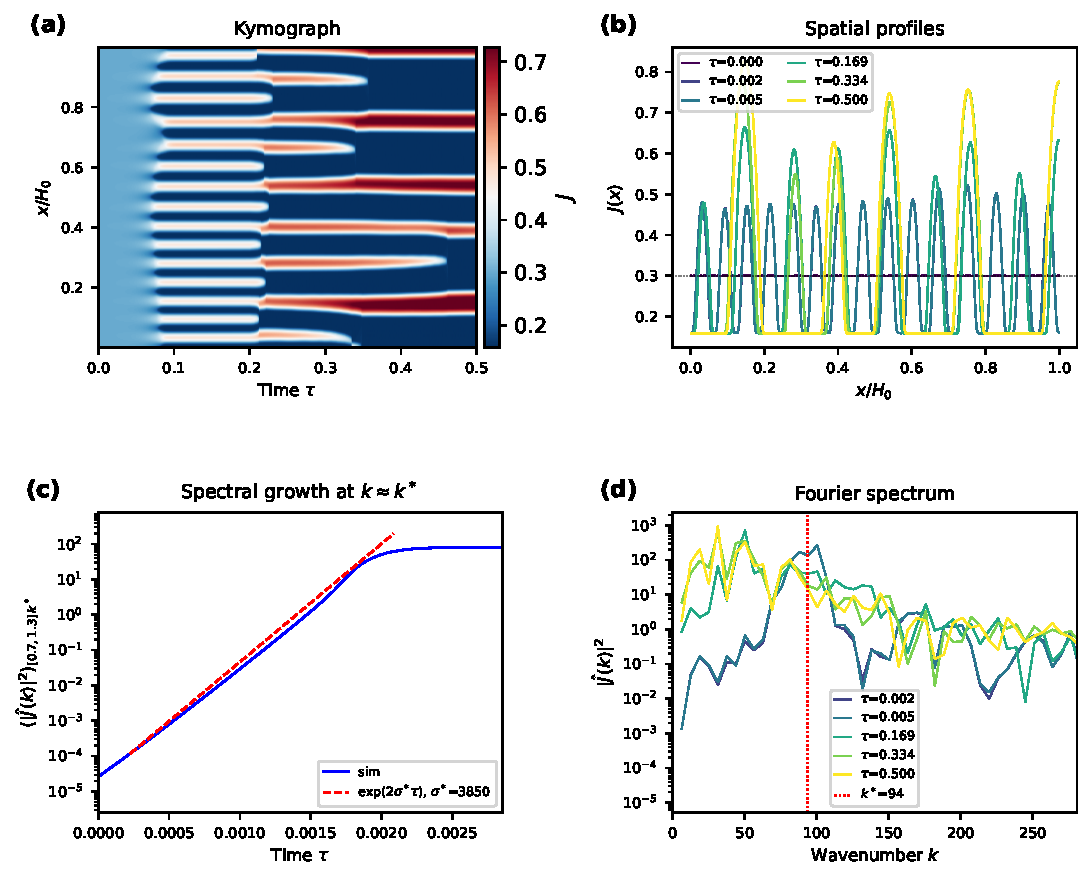
\includegraphics[width=\columnwidth]{fig7.pdf}
  \caption{Spinodal decomposition in the gel model with $\Da=0$
    (no reaction), $\theta=1.5$ (fixed), $J_0=0.30$,
    $\ell=0.01$, $N=301$, no-flux boundaries.
    \textbf{(a)}~Kymograph of $J(x,\tau)$ showing spontaneous
    domain formation and subsequent coarsening.
    \textbf{(b)}~Spatial profiles at selected times.
    \textbf{(c)}~Fourier amplitude $|\hat J(k^*)|^2$ averaged
    over $k\in[0.7k^*,1.3k^*]$; the predicted exponential growth
    at rate $2\sigma^*$ (red dashed) matches the simulation over
    five decades before nonlinear saturation.
    \textbf{(d)}~Fourier power spectrum $|\hat J(k)|^2$; the
    earliest curves peak near $k^*\!\approx 94$ (red dotted),
    shifting to lower $k$ during coarsening.}
  \label{fig:spinodal}
\end{figure}


\end{document}
